\chapter{Modélisation de la Forward Guidance et impact sur le stress systémique : le cas européen}
\minitoc

Après avoir introduit les fondements des architectures de réseaux neuronaux modernes, incluant les modèles Transformers, les SSM de type Mamba, LSTM et WAE l’accent avait été mis sur leur capacité à représenter de manière expressive et structurée les données séquentielles, tant textuelles que temporelles. C’est sur cette base méthodologique que s’appuie désormais l’exploration empirique, qui a pour objet principal de quantifier le rôle de la communication monétaire (en particulier la Forward Guidance) dans la dynamique du stress systémique européen mesuré par le CISS. Dans cette optique, un corpus textuel exhaustif a été constitué à partir des discours, déclarations et publications officielles de la BCE couvrant une période allant de janvier 2005 à décembre 2024. Ce corpus a été traité, encodé et analysé à l’aide de modèles de langage, permettant la construction d’un indicateur directionnel continu de Forward Guidance, capturant les nuances sémantiques des communications monétaires. Cette construction fait l’objet d’une section méthodologique dédiée dans laquelle sont décrites les étapes d’encodage, de projection vectorielle, de normalisation statistique, et d’évaluation comparative entre modèles linguistiques afin de choisir le meilleur score. L'objet de ce chapitre est donc d'évaluer si les déclarations de politique monétaire de la BCE 
mesurées par l'intensité de la FG accentuent ou atténuent le niveau de stress systémique en contrôlant les conditions macro-financières.\\

Le chapitre débute par une analyse statistique des données, à la fois du corpus textuel BCE et des indicateurs de stress systémique. Le traitement des discours inclut une exploration des volumes, de la longueur des documents et de leur distribution temporelle, mettant en évidence des pics de communication associés aux phases de crise. En parallèle, une série d’indicateurs de stress systémique, notamment les sous-composantes du CISS pour les marchés actions, monétaires et des changes, est analysée.
Des représentations graphiques et statistiques viennent illustrer la volatilité, les asymétries, et la co-mouvements de ces indicateurs au fil des chocs macro-financiers.\\

Une fois les données empiriques présentées, la construction de l’indicateur de FG est entreprise. Elle repose sur l’exploitation conjointe de plusieurs modèles de langage pré-entraînés (ModernBERT, Mamba, Mamba-2, Llamba) pour encoder chaque document en un vecteur dense, projeté ensuite sur un axe sémantique latent allant de la tonalité expansionniste à restrictive. Cet axe est défini à partir de phrases d’ancrage générées par des Large Language Models (LLaMA-3, Mistral 7B et Gemini), et validées selon une procédure rigoureuse. Un score directionnel est calculé pour chaque discours BCE puis normalisé, ce qui constitue une série temporelle de tonalité monétaire destinée à être exploitée dans les modèles d’impact. Une régression Ridge est alors mise en œuvre pour évaluer la capacité explicative de chaque version de l’indicateur sur le stress systémique, et pour sélectionner l’encodeur le plus performant à cette fin.\\

Le chapitre aborde ensuite la modélisation de l’impact de la Forward Guidance sur le stress systémique, en mobilisant une architecture neuronale WAE-LSTM. Deux variantes sont construites : un modèle conditionnel intégrant la FG comme signal exogène, et un modèle non conditionnel fondé uniquement sur les dynamiques internes des séries temporelles. Les fenêtres temporelles des données sont encodées, projetées dans un espace latent régularisé par la distance de Wasserstein, puis reconstruites via un LSTM. L’erreur de reconstruction obtenue est interprétée comme une mesure indirecte du stress latent, permettant de comparer l’effet différentiel de la FG dans la réduction du stress.\\

Les résultats empiriques sont ensuite présentés selon trois horizons temporels distincts. À court terme, la FG semble redondante, les marchés intégrant rapidement l’information disponible. Toutefois, des effets indirects sont mis en évidence : stabilisation des anticipations, réduction des asymétries d’information, ancrage comportemental. À moyen terme, l’effet de la FG devient plus complexe acec une efficacité qui baisse en période de crise, notamment en raison de la sémantique, d’une fragmentation du discours, ou d’un décalage entre intentions déclarées et politiques effectivement mises en œuvre. Le signal peut alors devenir instable, voire contre productif. À long terme, en revanche, un effet différé significatif est observé avec une FG apparaît comme un facteur explicatif robuste du stress latent, en raison de son rôle d’ancrage des anticipations, de crédibilité institutionnelle et de signal stratégique. Enfin, une section est consacrée aux recommandations opérationnelles à destination des régulateurs, en particulier de la BCE. Il y est proposé de renforcer la cohérence institutionnelle des discours, d’intégrer des dispositifs de suivi sémantique automatisé, d’internaliser les effets différés dans la stratégie de communication, et de mieux articuler la FG avec les instruments macroprudentiels et de liquidité. L’efficacité de la Forward Guidance est ainsi replacée dans une logique d’architecture intégrée de gestion des chocs financiers, où la parole n’est efficace que si elle est crédible, traçable et alignée sur les instruments. Il est ainsi ambitionné de démontrer que la FG, au-delà de son contenu discursif, peut être rigoureusement quantifiée dans une approche explicative du stress systémique.

\section{Analyse statistique des données}

L’analyse statistique des données constitue le point de départ de ce chapitre. Elle s’inscrit dans la continuité logique de l’approche méthodologique développée précédemment, en ancrant empiriquement les modèles présentés dans des jeux de données concrets. Ce paragraphe vise précisément à caractériser les données mobilisées dans l’étude, à la fois sur le versant textuel et sur le versant quantitatif via l’indicateur composite de stress systémique. D’abord, un corpus de textes a été constitué à partir des publications officielles de la BCE couvrant la période de janvier 2005 à décembre 2024. Cette base documentaire, extraite automatiquement par web scraping, regroupe l’ensemble des discours, communiqués et interventions institutionnelles. Chaque document a été structuré, horodaté et catégorisé, de manière à garantir une traçabilité complète et une compatibilité avec les techniques de traitement automatique du langage naturel. L’objectif est de permettre, in fine, l’encodage sémantique de la tonalité monétaire afin de construire un indicateur directionnel de Forward Guidance. Une première analyse statistique est réalisée pour apprécier la richesse, la diversité et l’évolution temporelle de cette communication. Ensuite, les données de stress systémique sont examinées à travers l’étude des sous-indicateurs du CISS relatifs aux marchés monétaires, actions et changes. Leur dynamique est analysée à la fois graphiquement et statistiquement, révélant des comportements hétérogènes selon les segments, mais également une forte interdépendance en période de crise. Ces observations serviront de socle à la modélisation ultérieure du stress latent, et permettront de mieux appréhender les canaux de transmission entre les signaux des discours de la BCE et la stabilité financière de la zone euro.

\subsection{Sources des données textuelles : discours et communiqués de la BCE}

Dans le cadre de la construction d’un indicateur quantitatif de FG, un corpus textuel étendu a été constitué à partir des publications officielles de la BCE. Cette base de données couvre une période allant de janvier 2005 à décembre 2024, permettant ainsi d’englober une diversité de régimes macro-financiers et monétaires (entre crises, normalisation et période déflationniste). Elle inclut notamment la grande crise financière de 2008, la crise des dettes souveraines européennes, la période de politique monétaire non conventionnelle marquée par des taux proches de zéro et des programmes d’achats d’actifs, la crise sanitaire mondiale liée au COVID-19, ainsi que la récente phase de resserrement des conditions monétaires face à la remontée de l’inflation.\\

La collecte des données textuelles a été réalisée par le biais d’une procédure automatisée de type \textit{web scraping}. À cette fin, un script Python a été développé, reposant sur l’utilisation de la bibliothèque \texttt{Selenium} mais aussi \texttt{BeautifulSoup}, laquelle permet d’interagir dynamiquement avec des pages web complexes. Le site institutionnel de la BCE a été exploré de manière systématique, ont été extraits l’ensemble des discours publics, déclarations officielles, communiqués de presse, conférences de presse post-réunion du Conseil des gouverneurs, ainsi que les interventions des membres du Directoire dans des forums, des conférences ou devant les parlements nationaux et européens. Chaque document a été conservé dans son intégralité, avec mention de la date, du lieu d’intervention, du type de document, et de l’intervenant (présidents successifs de la BCE à savoir Jean-Claude Trichet, Mario Draghi et Christine Lagarde ainsi que d’autres membres du Directoire).

Le corpus final ainsi constitué se compose de 3005 documents avant alignement temporel, représentant plusieurs millions de mots. Afin d’apprécier empiriquement la diversité et la complexité de ce corpus, des statistiques descriptives ont été établies sur la longueur des documents (mesurée en nombre de mots). Les résultats sont présentés dans le \autoref{tab:stats_des_textes} :

\begin{table}[H]
\centering
\begin{tabular}{lr}
\toprule
\textbf{Statistique} & \textbf{Valeur} \\
\midrule
Nombre de documents analysés & 3005 \\
Longueur moyenne             & 2239 \\
Écart-type                   & 1557 \\
Minimum                      & 44 \\
1er quartile (Q1)            & 1117.0 \\
Médiane (Q2)                 & 1907.0 \\
3e quartile (Q3)             & 3184.0 \\
Maximum                      & 5809 \\
\bottomrule
\end{tabular}
\caption{Statistiques descriptives de la longueur des documents BCE (en nombre de mots)}
\label{tab:stats_des_textes}
\end{table}

Il est ainsi observé une forte hétérogénéité dans les longueurs des documents. Certains sont relativement courts, souvent de simples communiqués de presse ou réponses brèves à des questions, tandis que d'autres atteignent plusieurs milliers de mots, typiquement dans le cas des conférences de presse post-réunion ou des discours structurés du président de la BCE. La médiane de 1907 mots suggère un volume tout de même conséquent pour une majorité de publications, ce qui reflète le caractère argumentatif et technique de la communication de politique monétaire. Enfin, une analyse du corpus permet de mettre en évidence les fluctuations du volume de communication institutionnelle dans le temps. La \autoref{fig:nb_docs_par_annee} suivante illustre le nombre de documents publiés chaque année entre 1998 et 2025 :

\begin{figure}[H]
    \centering
    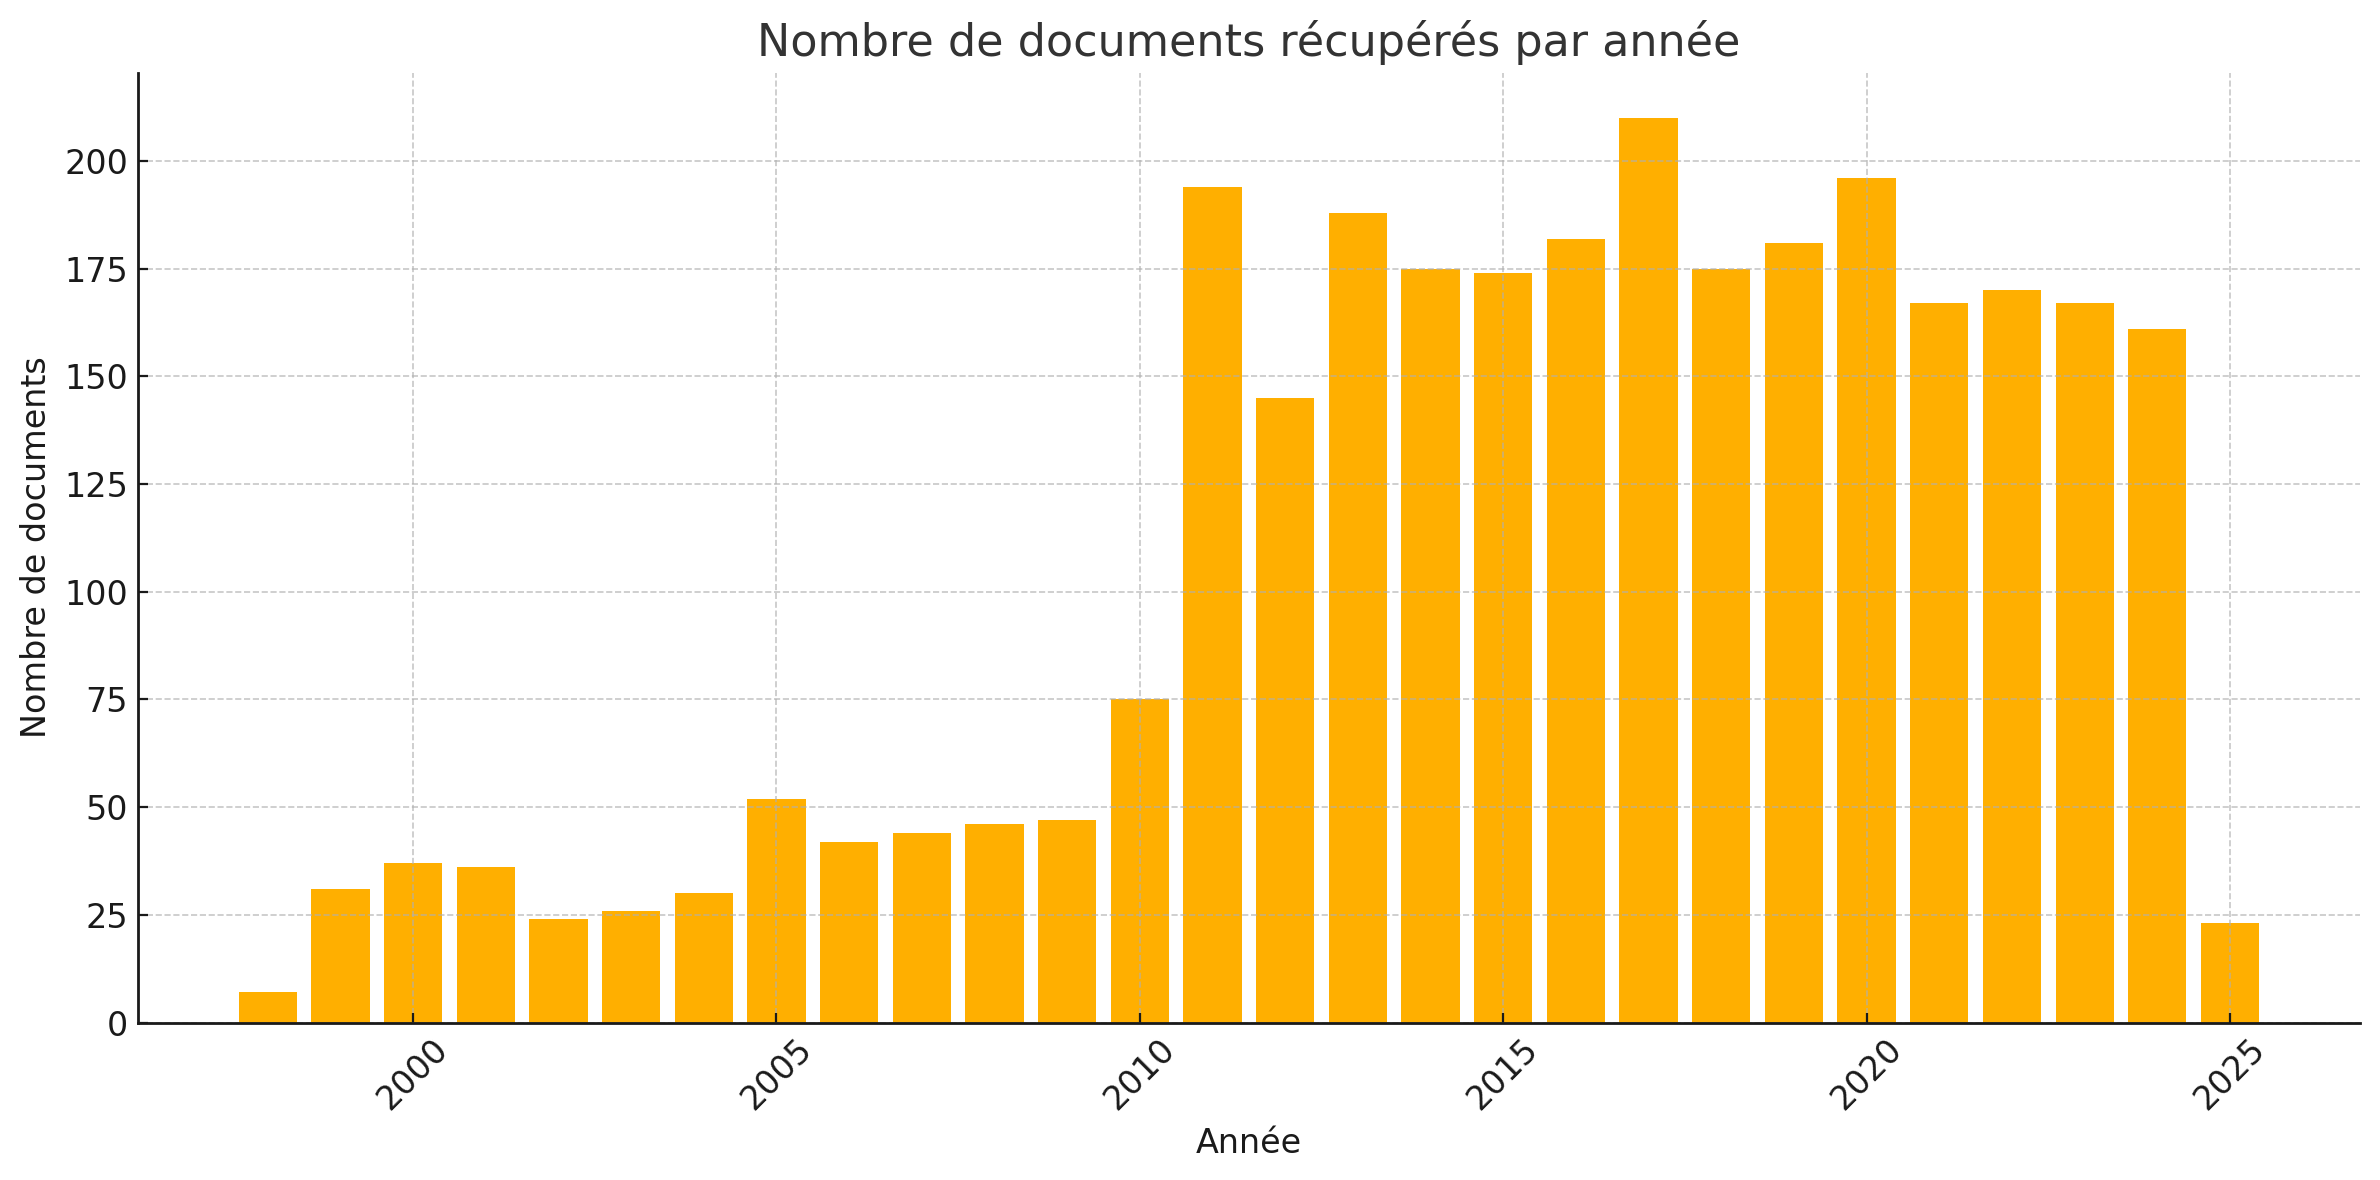
\includegraphics[width=0.9\linewidth]{images/docs_par_annee.png}
    \caption{Nombre de discours et communiqués publiés par la BCE par année (2005–2024)}
    \label{fig:nb_docs_par_annee}
\end{figure}

Il est possible de repérer visuellement plusieurs pics d’activité, généralement corrélés à des périodes de tensions financières ou de révisions majeures de l’orientation monétaire. Ces observations confirment que la fréquence et la densité des discours peuvent elles-mêmes constituer des variables d’intérêt dans l’étude du rôle de la Forward Guidance. Elles suggèrent également l’existence de liens potentiels entre l’intensité de la communication monétaire et les épisodes de stress financier. Afin d’explorer ces liens de manière plus systématique, il convient désormais d’analyser les données relatives au stress systémique, en s’appuyant sur les sous-composantes du CISS, qui mesurent les tensions observées sur les principaux segments des marchés financiers.


\subsection{Données de stress systémique : CISS et sous-composantes}

L'évolution des sous-indicateurs de stress des trois principaux segments financiers : le marché monétaire, le marché des actions et le marché des changes est analysé sous un angle graphique dans la \autoref{fig:graphindicateurs} puis par rapport aux statistiques descriptives dans le \autoref{fig:statsdescriptives}.

\begin{figure}[H]
    \centering
    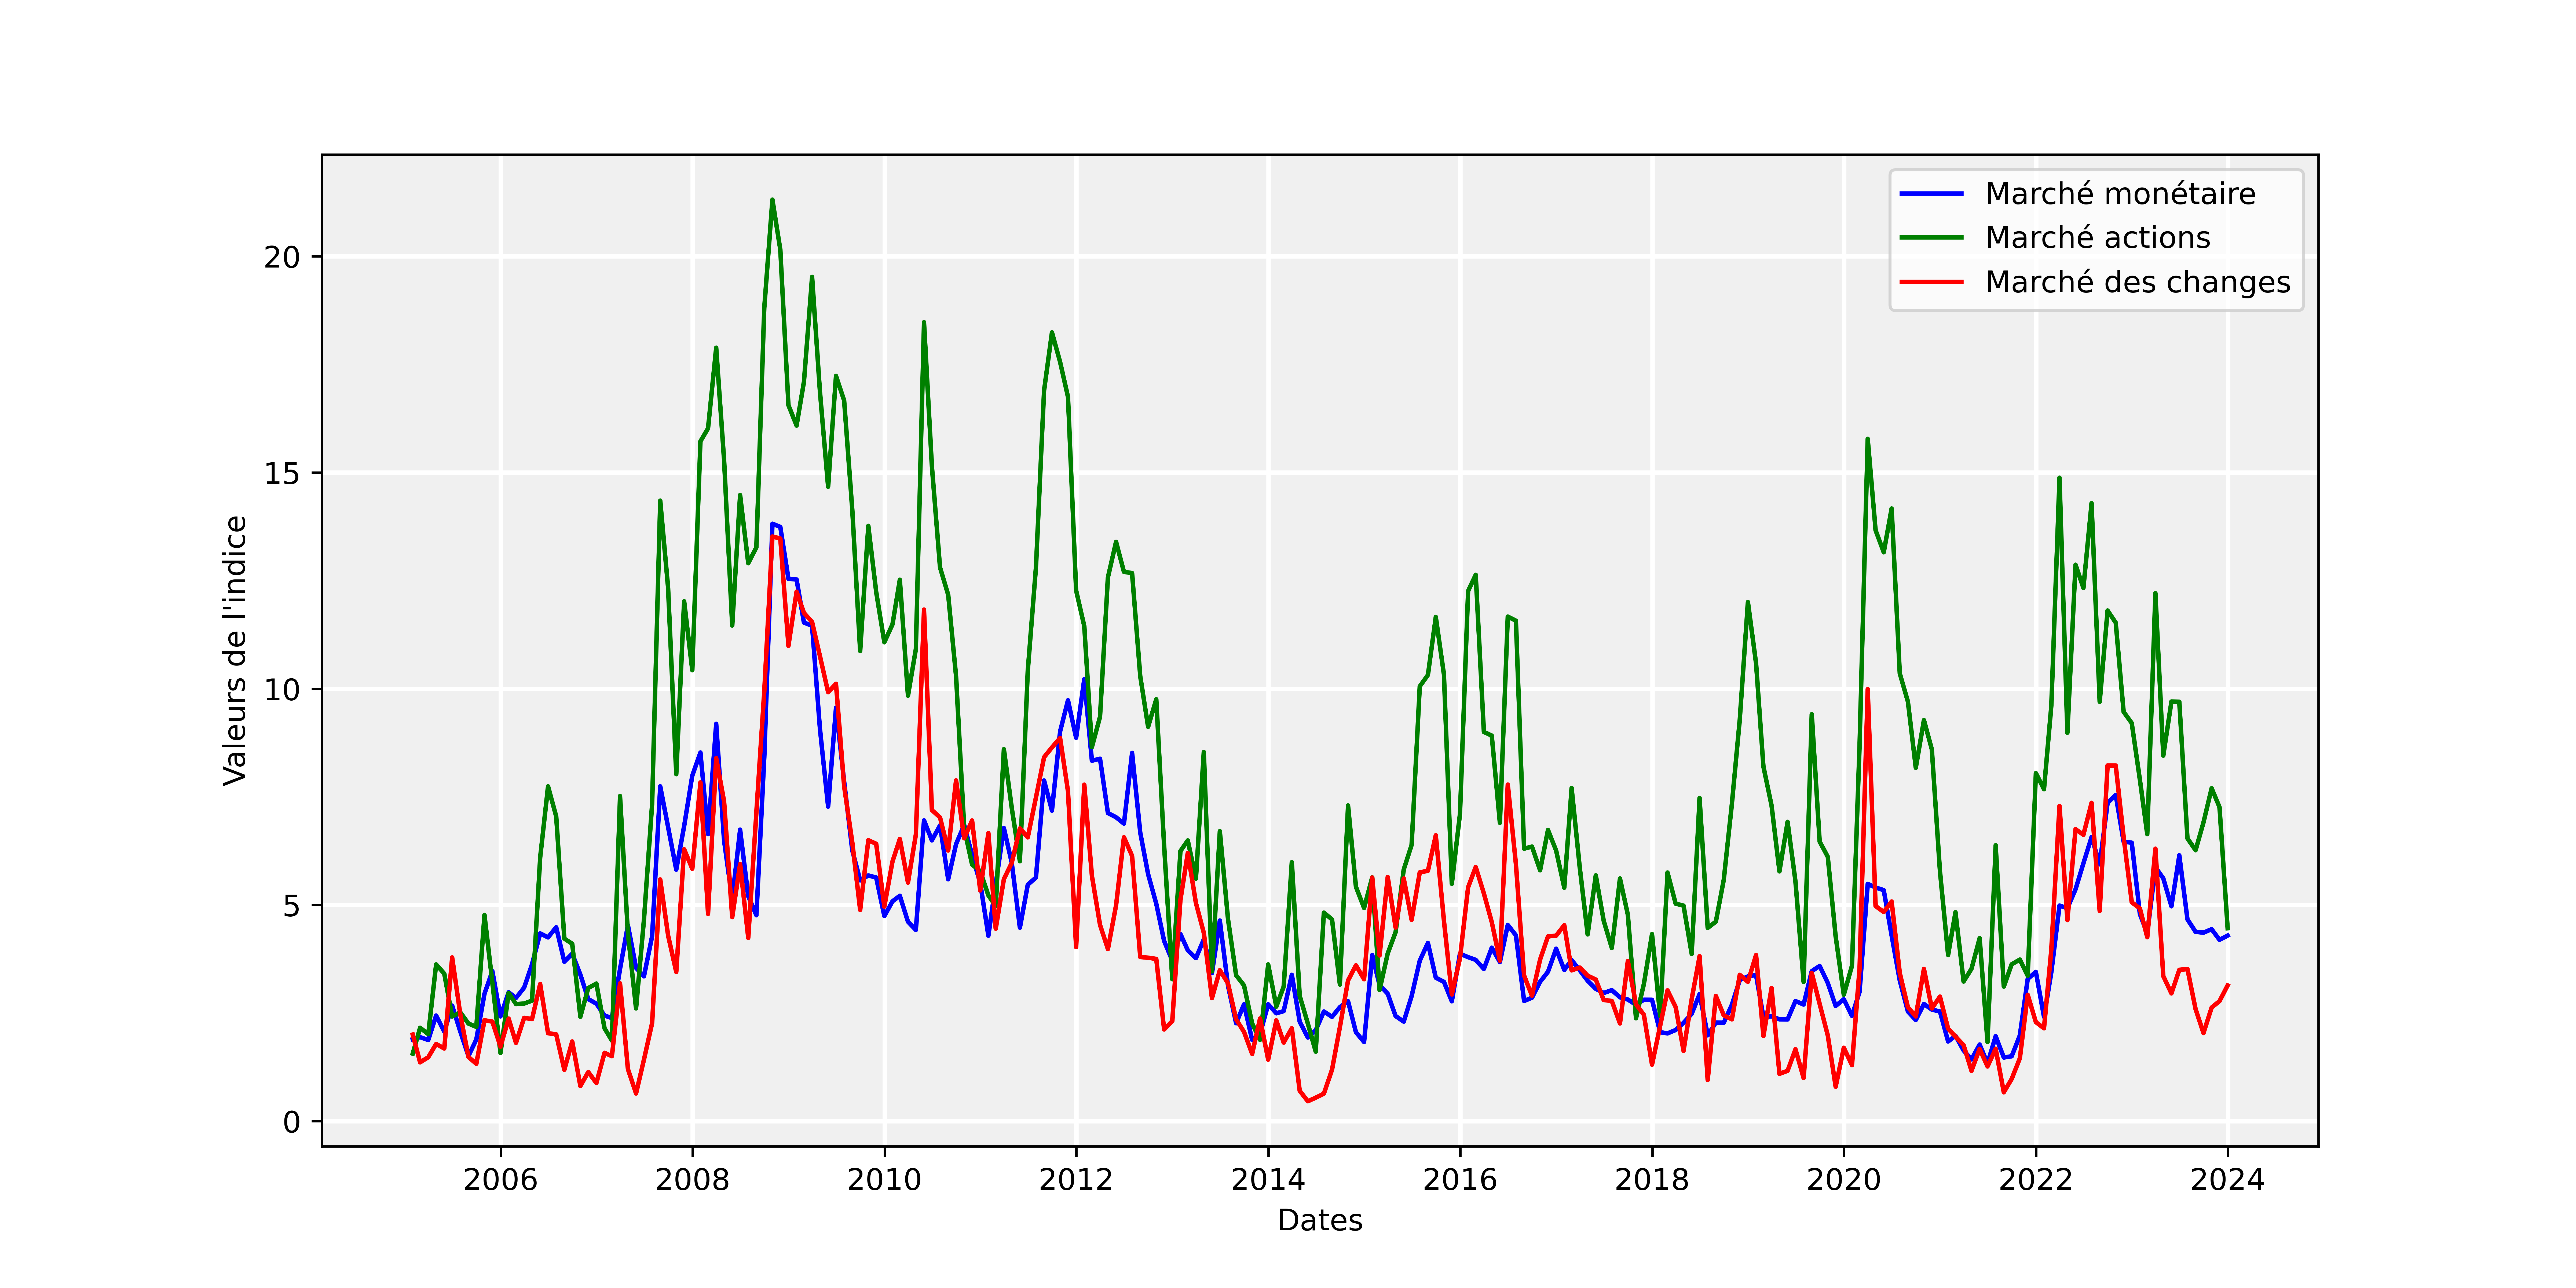
\includegraphics[width=1\linewidth]{images/sous_indicateurs_stress.png}
    \caption{Sous-indicateurs de stress entre janvier 2005 et décembre 2024.}
    \label{fig:graphindicateurs}
\end{figure}

Le graphique montre l'évolution des sous-indicateurs de stress des trois principaux segments financiers (marché monétaire, marché des actions, et marché des changes) entre janvier 2005 et décembre 2024. Chaque indicateur est représenté par une courbe distincte : le marché monétaire est en bleu, le marché des actions en vert, et le marché des changes en rouge.\\

Le marché des actions montre la plus grande volatilité parmi les trois indicateurs. À plusieurs reprises, notamment entre 2008 et 2012 ainsi que vers 2020, des pics marqués, correspondant à des périodes de forte tension sur ce marché. Le stress sur le marché des actions est particulièrement élevé lors des crises financières, comme celle de 2008, où le graphique montre une nette augmentation du stress. Après cette période de crise, le stress sur le marché des actions diminue progressivement, bien que des pics sporadiques apparaissent, notamment en 2020, ce qui pourrait être attribué à la crise liée à la pandémie de COVID-19. En général, la courbe verte représente des variations assez brusques, ce qui reflète la nature plus volatile du marché des actions, particulièrement sensible aux événements macroéconomiques et aux changements dans les conditions du marché mondial.

\begin{figure}[H]
    \centering
    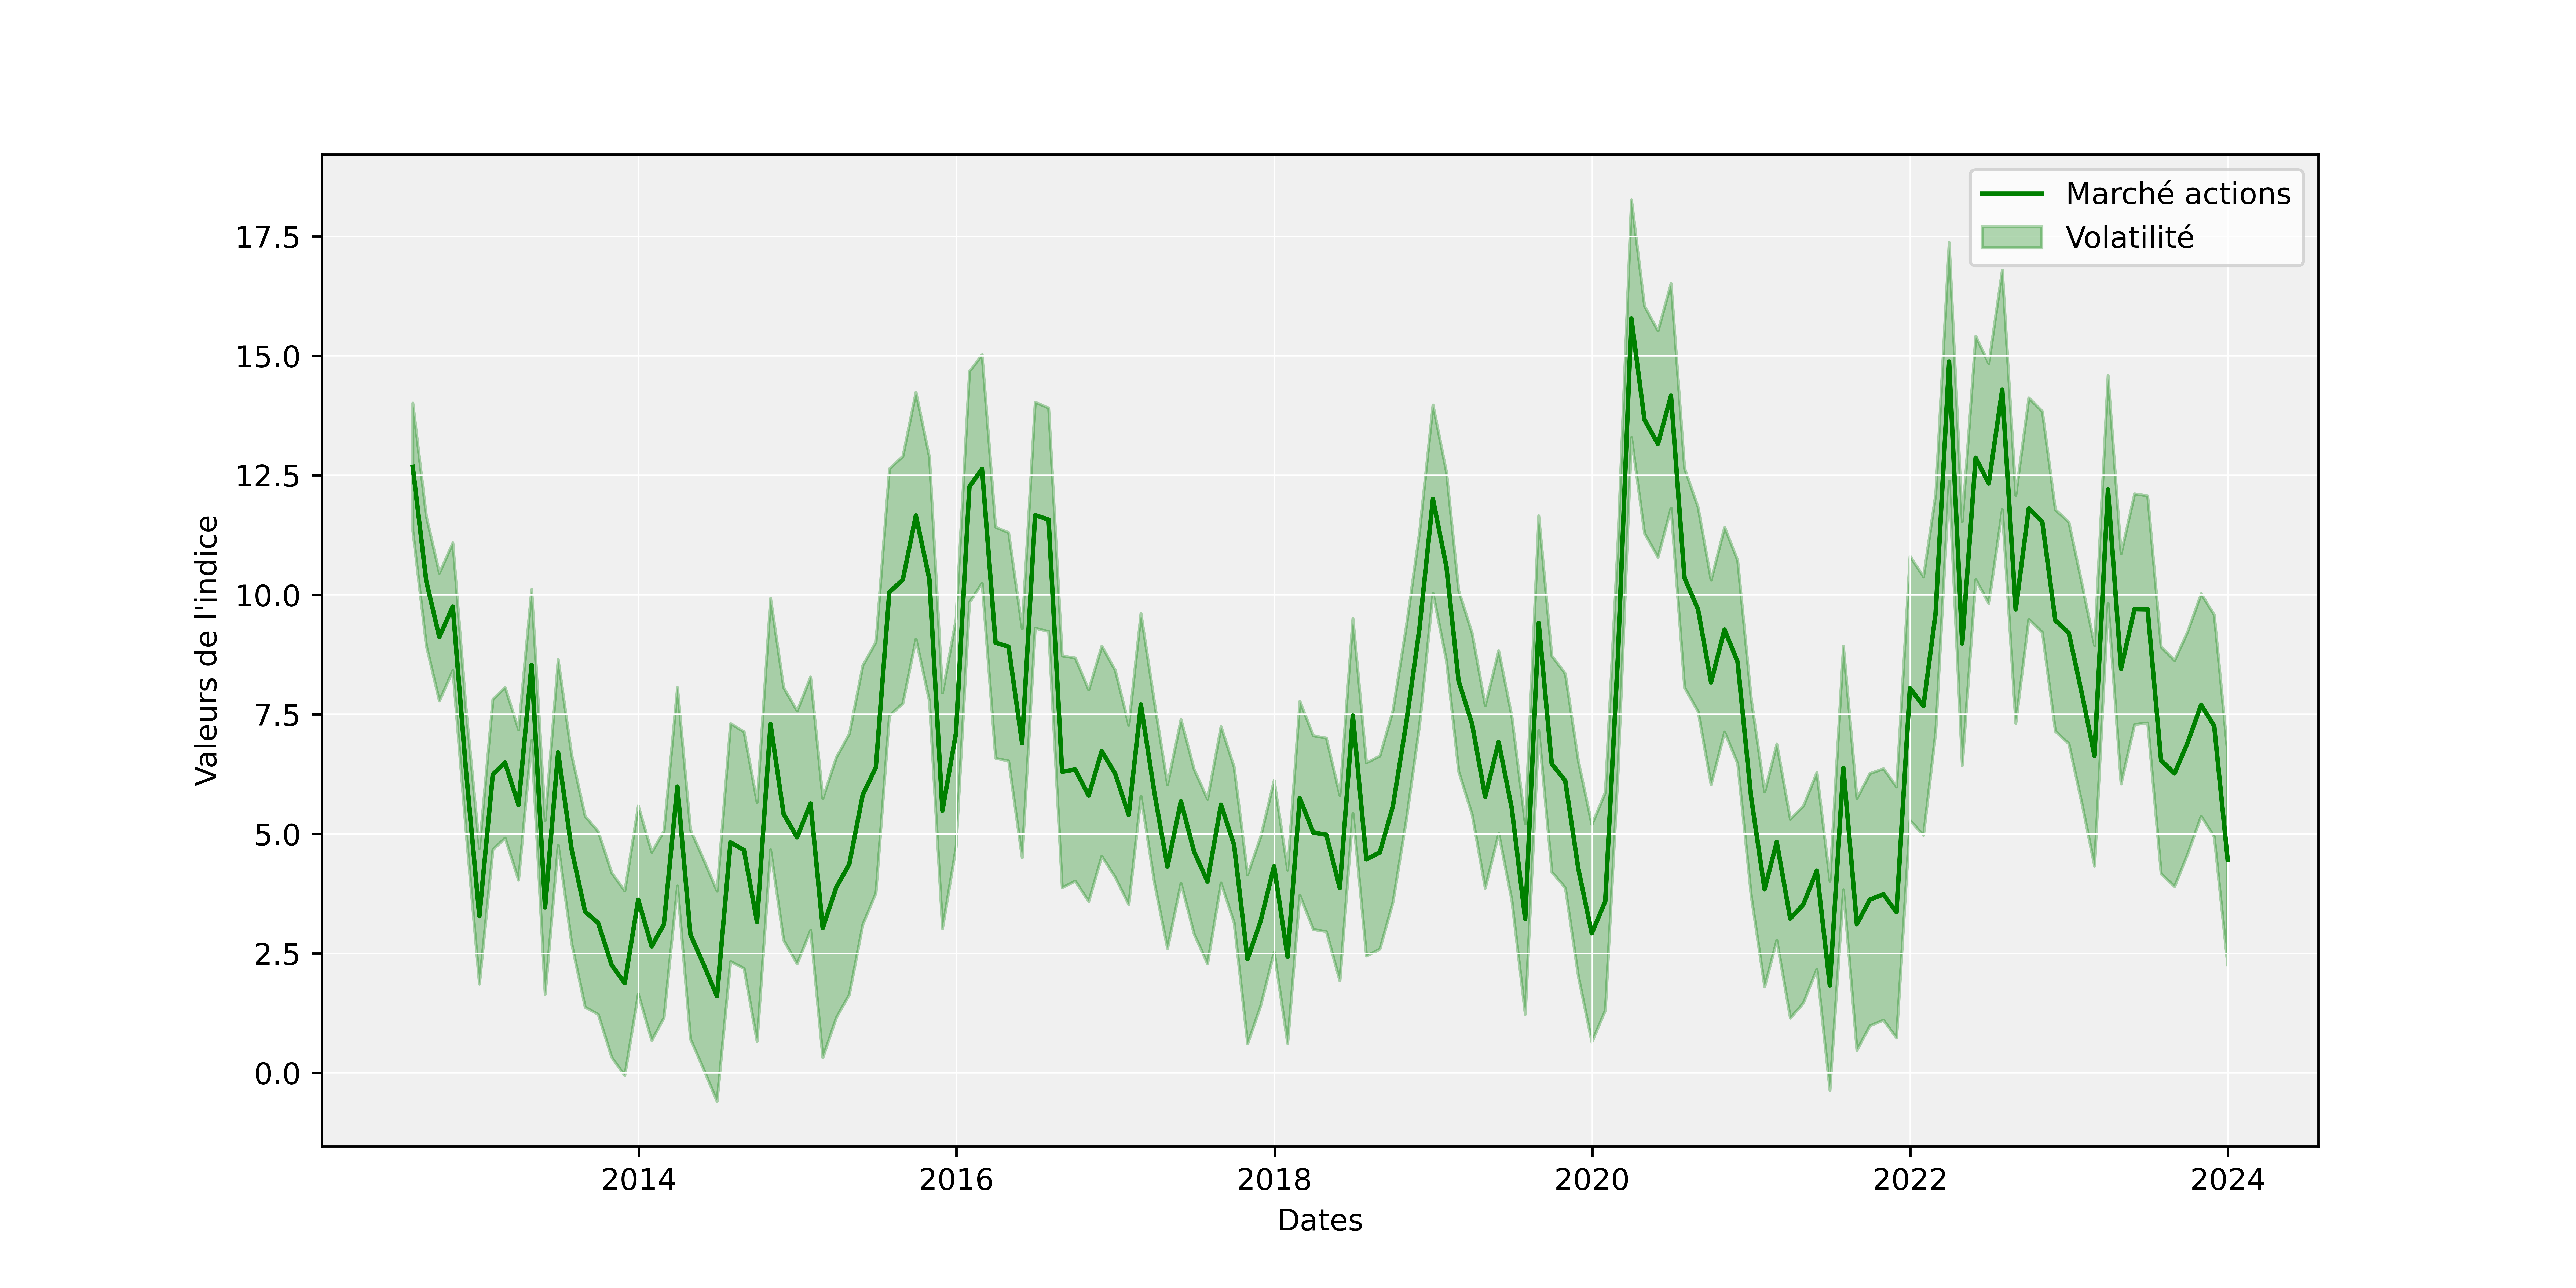
\includegraphics[width=1\linewidth]{images/sous_indicateurs_equity_stress_equity.png}
    \caption{Stress sur le marché actions et volatilité associée entre janvier 2005 et décembre 2024.}
    \label{fig:enter-label}
\end{figure}

La volatilité observée sur le marché des actions suggère que les investisseurs réagissent fortement aux événements qui affectent la confiance dans les entreprises et l’économie en général. Les pics de volatilité élevés, particulièrement en 2008 et 2020, indiquent que les actions subissent des ajustements massifs des portefeuilles des investisseurs, souvent en raison de ventes paniquées ou de changements rapides dans les perspectives économiques.\\

En ce qui concerne le marché monétaire, cela montre des variations plus modérées par rapport aux autres marchés. Bien qu’il y ait des pics de stress, notamment autour des crises financières majeures, les valeurs de l'indicateur restent globalement plus stables. Cela reflète la nature plus régulée et contrôlée du marché monétaire, où les banques centrales interviennent régulièrement pour stabiliser les conditions de liquidité. Il est possible d'observer des pics importants autour de 2008 et un autre vers 2012, correspondant à la crise de la dette souveraine en Europe, ainsi que de légères hausses durant d'autres périodes de tension comme la crise de 2020. Cependant, contrairement au marché des actions, le marché monétaire retourne rapidement à des niveaux de stress plus bas après ces périodes de tension. Cela montre une capacité de stabilisation plus rapide dans ce segment du marché.

\begin{figure}[H]
    \centering
    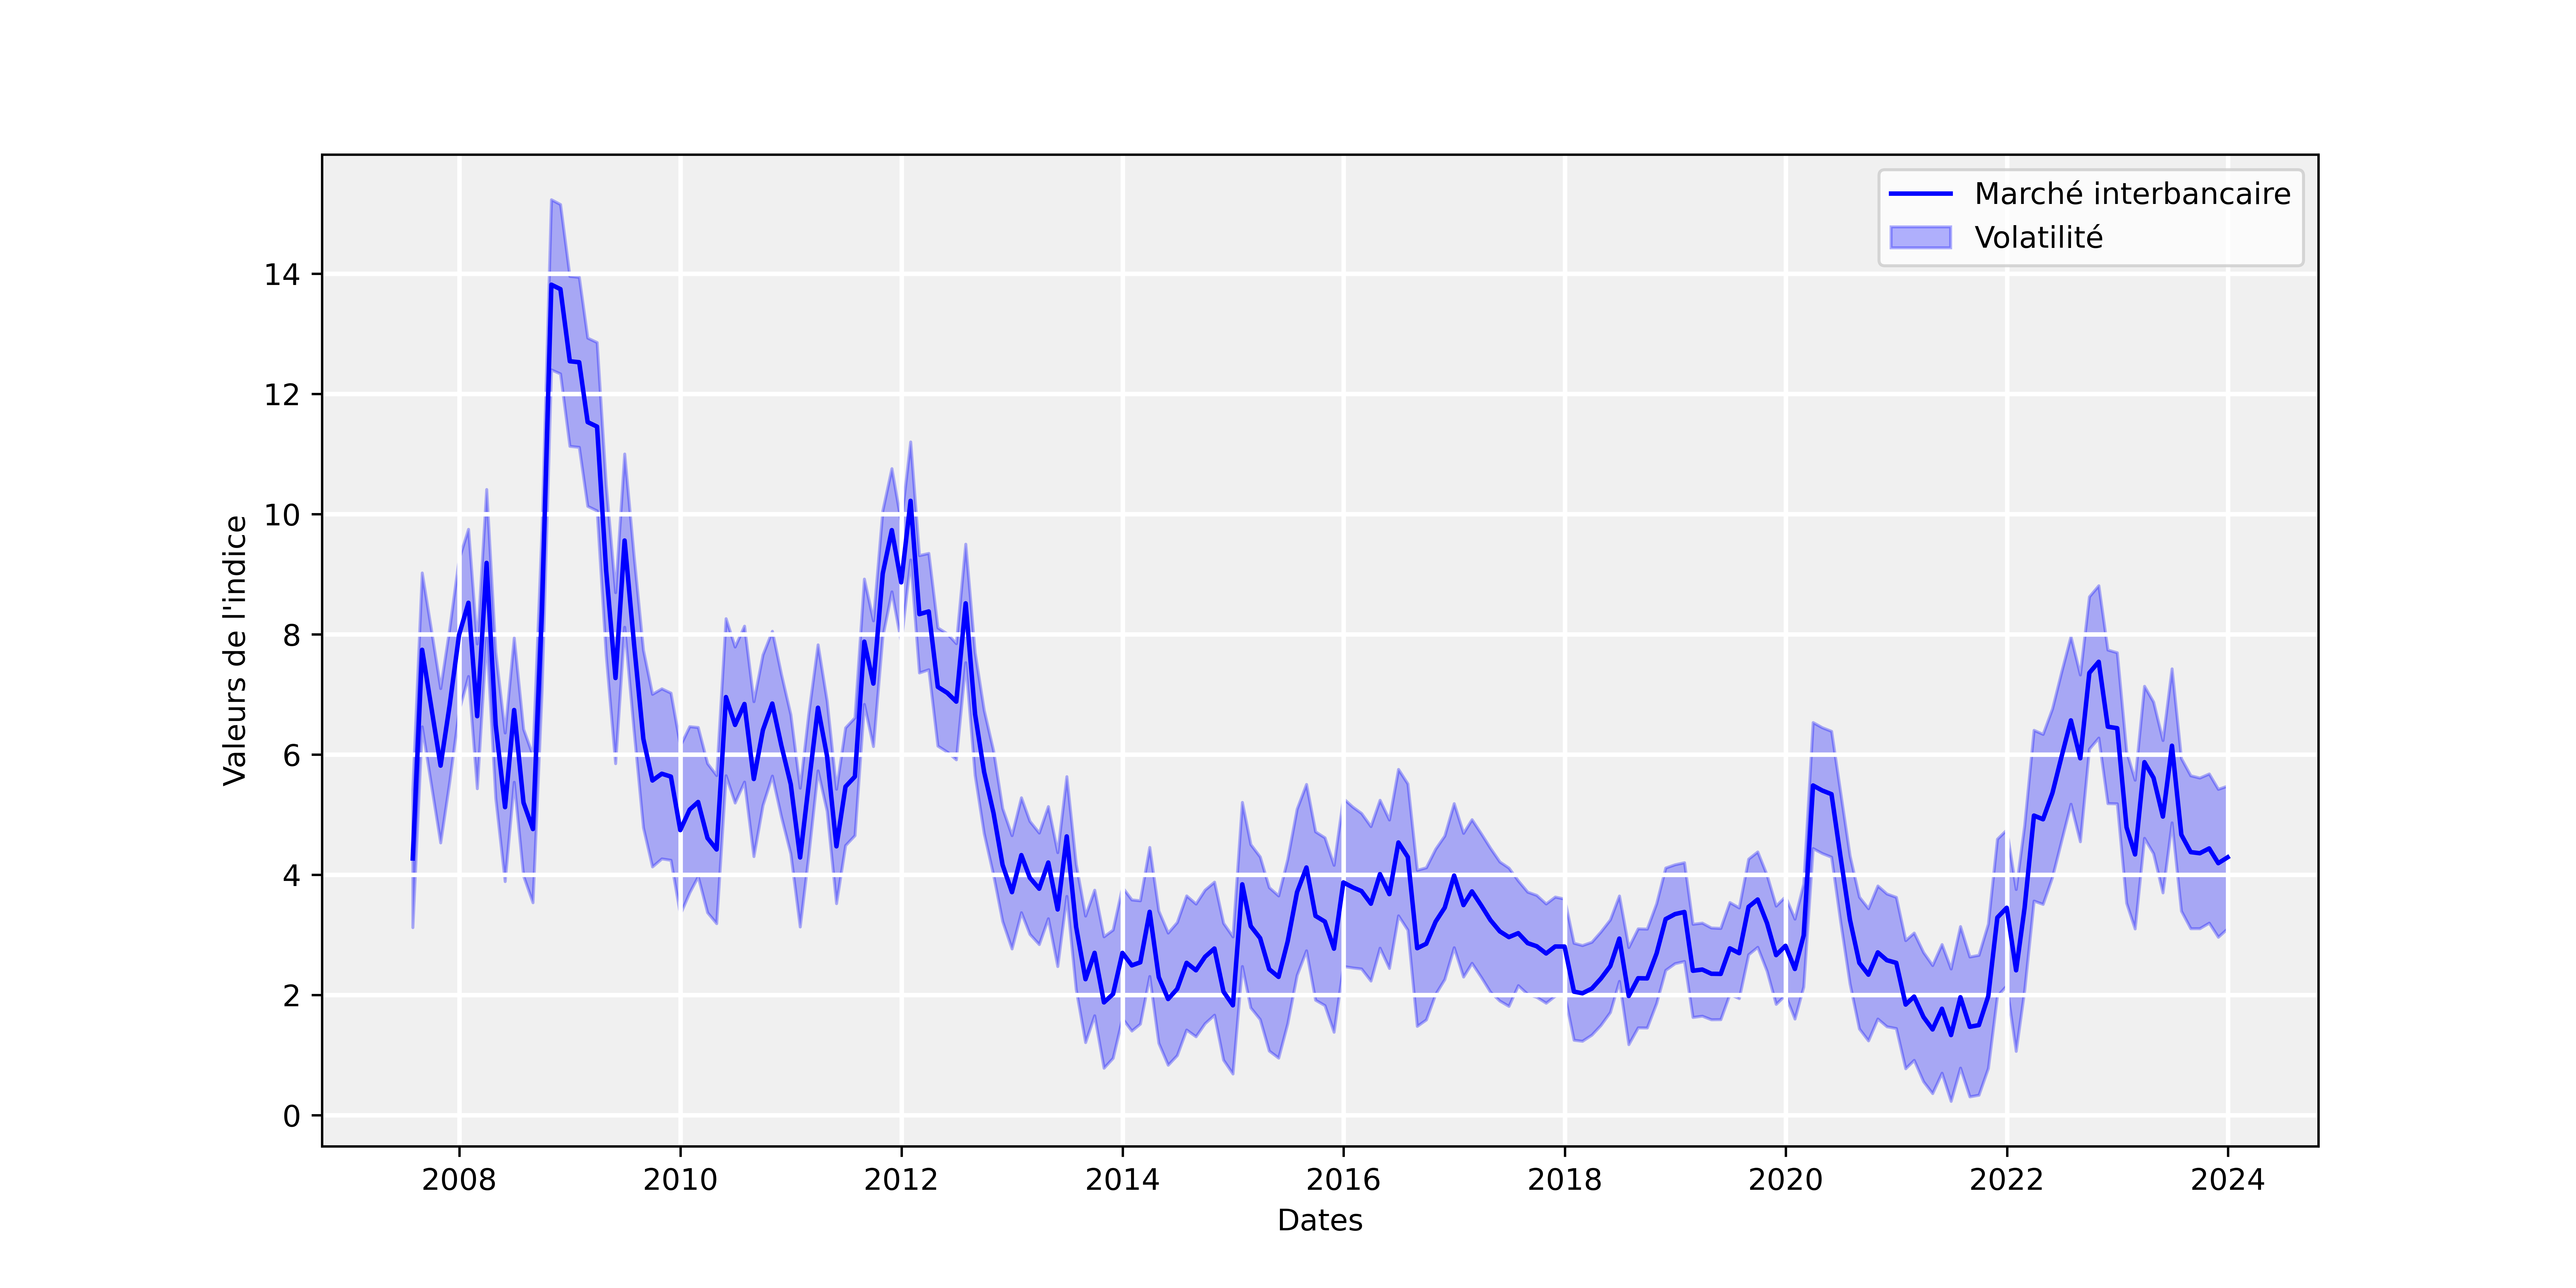
\includegraphics[width=1\linewidth]{images/sous_indicateurs_stress_imm.png}
    \caption{Stress sur le marché monétaire et volatilité associée entre janvier 2005 et décembre 2024.}
    \label{fig:enter-label}
\end{figure}

La volatilité modérée associée au stress sur le marché monétaire, par rapport au marché des actions, est en partie due à la capacité des banques centrales à stabiliser ce marché via leurs outils de politique monétaire. Les pics de volatilité, en particulier en 2008 et 2011, sont le reflet des périodes où les banques hésitent à se prêter mutuellement, indiquant un risque accru de crise de liquidité. Cependant, après les interventions des régulateurs, la volatilité diminue rapidement, témoignant de la résilience de ce marché.\\

Enfin, le marché des changes est globalement le moins stressé parmi les trois segments, comme en témoignent les niveaux relativement bas de la courbe rouge. Cependant, ce marché montre également des épisodes de stress ponctuels, en particulier autour de 2008 et 2010-2012, ainsi que quelques augmentations notables dans les années plus récentes (vers 2020). La nature décentralisée et liquide du marché des changes lui permet de mieux absorber les chocs, bien que des périodes de forte volatilité, notamment causées par les fluctuations des taux de change et les crises monétaires, entraînent des pics soudains. Le stress sur ce marché semble être plus transitoire et moins soutenu que sur le marché des actions, où les tensions persistent souvent sur une plus longue période.

\begin{figure}[H]
    \centering
    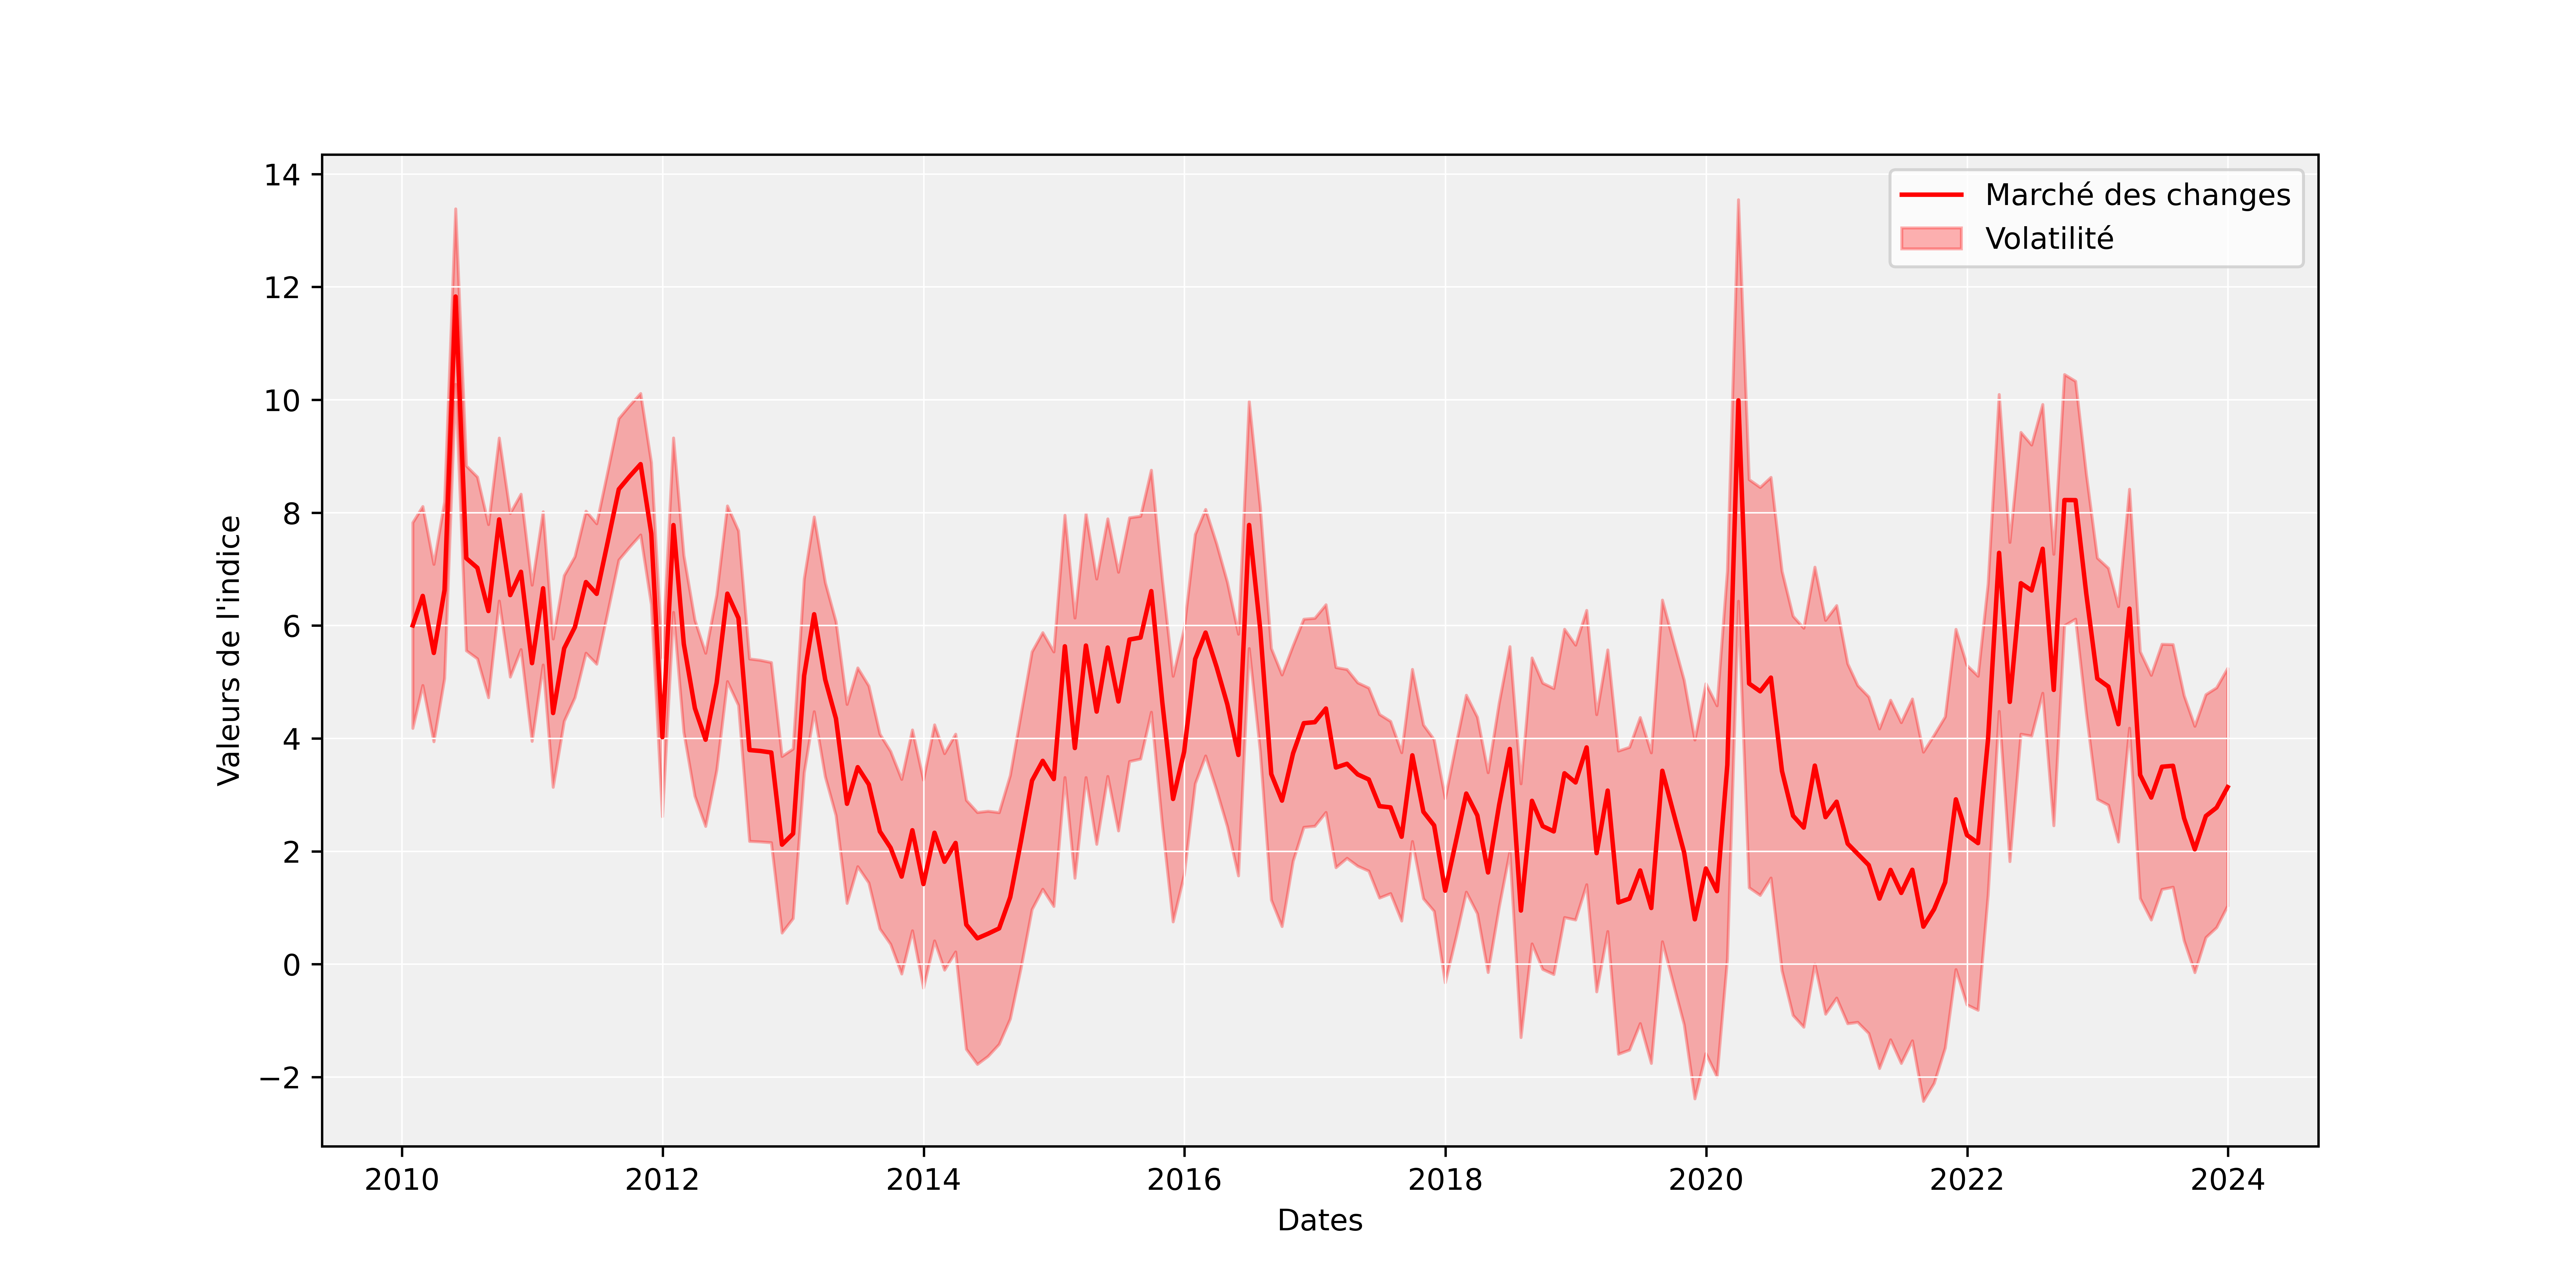
\includegraphics[width=1\linewidth]{images/sous_indicateurs_forex_stress_forex.png}
    \caption{Stress sur le marché des changes et volatilité associée entre janvier 2005 et décembre 2024.}
    \label{fig:enter-label}
\end{figure}

La volatilité, qui accompagne les hausses de stress, est particulièrement importante autour de ces périodes. Les fluctuations observées en 2020 peuvent être attribuées aux mouvements des taux de change lors de la pandémie, ainsi qu'à la réponse des banques centrales à travers des ajustements des taux d'intérêt et des mesures non conventionnelles. Cependant, même si des périodes de stress apparaissent, le marché des changes tend à revenir à des niveaux de stress modérés sur le long terme, reflétant sa capacité à absorber les chocs grâce à sa liquidité élevée et à son caractère global.\\

En somme, l'interconnexion entre ces trois indicateurs de stress est bien visible. Lors des grandes crises financières, comme celle de 2008, on observe des pics simultanés dans les trois indicateurs, ce qui reflète un stress systémique à travers plusieurs segments financiers. Cependant, chaque marché semble réagir différemment en fonction de sa structure et de sa régulation. Le marché des actions tend à subir des chocs plus fréquents et plus sévères, tandis que le marché des changes montre une capacité à absorber les chocs avec des variations moins marquées. Le marché monétaire, quant à lui, présente une stabilité relative, malgré des tensions durant les périodes de crise.\\

Cette analyse démontre l'importance de surveiller l'évolution simultanée des sous-indicateurs de stress pour comprendre comment les tensions dans un segment peuvent se propager aux autres, exacerbant ainsi les crises financières. Après avoir effectué une analyse graphique des sous-indicateurs de stress pour les trois principaux segments financiers, l'analyse des statistiques descriptives va être menée. Cette approche permettra de mieux comprendre la distribution et les caractéristiques des différents indicateurs de stress en quantifiant leur tendance centrale, leur dispersion.

\begin{table}[H]
    \centering
    \sffamily
    \scalebox{0.9}{\begin{tabular}{lccccccc}
        \toprule
        \textbf{Indicateurs} & \textbf{Moyenne} & \textbf{Médiane} & \textbf{Maximum} & \textbf{Minimum} & \textbf{Écart-type} & \textbf{Skewness} & \textbf{Kurtosis} \\
        \midrule
        IMM      & 4.39  & 3.68  & 13.82  & 1.33  & 2.38  & 1.45  & 5.35  \\
        FOREX    & 4.19  & 3.52  & 13.52  & 0.46  & 2.65  & 1.09  & 4.07  \\
        EQUITY   & 8.02  & 6.91  & 21.31  & 1.56  & 4.56  & 0.68  & 2.64  \\
        \bottomrule
\end{tabular}
}
    \caption{Statistiques descriptives.}
    \label{fig:statsdescriptives}
\end{table}

L'analyse des moyennes montre que l'indicateur de stress sur le marché des actions  présente la valeur moyenne la plus élevée avec 8.02, suivie par les marchés interbancaire et des changes avec des moyennes respectives de 4.39 et 4.19. Cela suggère que, dans l'ensemble, le marché des actions tend à subir un stress plus important que les marchés des changes et interbancaire. En observant les valeurs médianes, il est possible de voir que le marché des actions affiche également la valeur médiane la plus élevée (6.91), ce qui renforce l'idée que ce marché est plus fréquemment sujet à des périodes de stress élevé. Les marchés interbancaire et des changes ont des valeurs médianes plus proches de leur moyenne, respectivement à 3.68 et 3.52, ce qui indique une distribution des données plus symétrique, bien que des périodes de stress aigu existent.\\

Les valeurs maximales et minimales montrent que marché des actions a connu des pics de stress beaucoup plus élevés, avec une valeur maximale de 21.31, contre 13.82 pour l'IMM et 13.52 pour le FOREX. De plus, les valeurs minimales montrent que le marché des changes a subi des périodes de stress très faibles avec une valeur minimale de 0.46, beaucoup plus basse que celles observées sur les marchés interbancaire (1.33) et des actions (1.56). Cela suggère que le marché des changes est potentiellement plus volatil avec des périodes de très faible stress ainsi que des pics de stress relativement élevés.

\newpage

L'écart-type permet de mesurer la dispersion des données autour de la moyenne, il est aussi une mesure de la volatilité. L'indicateur de stress du marché des actions présente une dispersion plus large (4.56), indiquant une plus grande volatilité des niveaux de stress par rapport aux autres marchés. Le FOREX montre également une volatilité non négligeable avec un écart-type de 2.65, tandis que l'IMM affiche la plus faible volatilité avec 2.38.\\

En examinant les coefficients d'asymétrie, tous les indicateurs présentent une asymétrie positive, ce qui signifie que les périodes de stress extrême sont plus fréquentes du côté des valeurs élevées. Le marché interbancaire présente la plus forte asymétrie (1.45), ce qui indique que ce marché connaît des épisodes de stress élevé relativement rares mais intenses. Le FOREX est également assez asymétrique avec une valeur de 1.09, tandis que le marché des actions présente une asymétrie plus modérée avec un coefficient de 0.68. Enfin, les coefficients de kurtosis montrent des informations sur la forme de la distribution des stress. Le marché interbancaire présente une kurtosis de 5.35, ce qui indique une distribution leptokurtique, caractérisée par des extrêmes plus fréquents et des périodes de stress aigu prononcées. Le FOREX affiche également une kurtosis élevée à 4.07, tandis que le marché des actions présente une distribution plus aplatie (2.64), indiquant une distribution plus proche de la normale.\\

Cela montre donc que le marché des actions tend à subir un stress plus élevé et plus volatil que les marchés des changes et interbancaire. Cependant, les périodes de stress intense sur le marché interbancaire se caractérisent par des épisodes plus rares mais plus extrêmes, comme le montrent ses valeurs de skewness et de kurtosis.

\subsection{Alignement temporel et granularité}

Afin de permettre une analyse cohérente entre les discours de la BCE et les indicateurs de stress financier, un alignement temporel des séries de données a été mis en œuvre. Les deux ensembles (textuel et quantitatif) ont été synchronisés à une fréquence hebdomadaire, considérée comme le compromis optimal dans le cadre de l’analyse de la politique monétaire et de l’impact de la Forward Guidance. Cette granularité permet de capturer des dynamiques suffisamment fines sans être affectées par le bruit de haute fréquence, tout en assurant une représentation temporelle compatible avec le rythme des communications institutionnelles et les évolutions des marchés financiers.\\

Pour chaque date hebdomadaire correspondant à une observation du CISS (de janvier 2005 à décembre 2024), un discours de la BCE a été associé selon une règle précise : si plusieurs discours étaient disponibles durant la semaine, celui correspondant exactement à la date d’observation du CISS était privilégié. En l’absence de discours à cette date, le discours le plus proche dans le passé (mais jamais postérieur) a été sélectionné. Ce choix méthodologique garantit une stricte antériorité du signal discursif par rapport à l’indicateur de stress, condition nécessaire pour préserver la validité causale dans les analyses ultérieures. Du côté des données quantitatives, les sous-indicateurs de stress extraits du CISS sont directement exploitables à fréquence hebdomadaire, sans nécessité d’agrégation supplémentaire. L’ensemble du dispositif aboutit ainsi à la constitution de couples temporels $(X_t, y_t)$, où $X_t$ désigne le discours institutionnel sélectionné à la date $t$ et $y_t$ la valeur du stress systémique observée cette même semaine. Cette construction permet une mise en correspondance rigoureuse des données textuelles et numériques, indispensable pour évaluer de manière crédible l’impact différé de la Forward Guidance sur la stabilité financière.\\

En définitive, l’analyse statistique exploratoire menée a permis de caractériser en détail les deux piliers empiriques du présent mémoire : d’une part, la structure et la temporalité des discours officiels de la Banque Centrale Européenne ; d’autre part, la dynamique et la distribution des tensions financières captées par les sous-indicateurs du CISS. La mise en lumière des régularités statistiques propres à chaque segment constitue une étape préparatoire à la modélisation intégrée. Elle justifie notamment le recours à des approches capables de capturer simultanément les dimensions sémantiques de la communication monétaire et les réponses structurelles des marchés. C’est dans cette perspective que s’ouvre désormais le paragraphe suivant, consacrée à la construction d’un indicateur directionnel de FG. À partir du corpus textuel analysé, il s’agira de quantifier, à l’aide de modèles de langage avancés, la tonalité implicite des discours de la BCE sur un axe allant de l’accommodant au restrictif. Cette mesure permettra d’intégrer la dimension sémantique de la politique monétaire dans un cadre de modélisation dynamique du stress systémique.

\section{Construction de l’indicateur de Forward Guidance}

Précédemment, il a été posé les fondations empiriques de ce travail, en décrivant la structure des données textuelles issues des publications de la BCE ainsi que les dynamiques observées des tensions financières à travers les composantes du CISS. Cette double caractérisation met en évidence la nécessité de relier de manière formalisée le contenu sémantique de la communication monétaire aux évolutions du stress systémique. Dans cette optique, ce paragraphe introduit une méthodologie de construction d’un indicateur directionnel de FG, fondé sur des techniques d’apprentissage profond appliquées au traitement automatique du langage. L’objectif est de transformer des discours non structurés en une variable continue, reflétant le ton monétaire implicite véhiculé par la BCE au fil du temps. L’approche adoptée combine la richesse contextuelle des modèles transformeurs de dernière génération avec la simplicité interprétative d’un axe latent construit à partir d’exemples de référence générés par LLM. Trois LLM ont été choisis : Llama 3, Mistral 7B et Gemini. Chaque phrase $x$ est d’abord encodée en un vecteur dense de dimension $d$ grâce à ModernBERT, Mamba, Mamba-2 et Llamba. Elle est ensuite projetée sur un vecteur directionnel $\hat V$ obtenu par différence entre phrases canoniquement expansives et restrictives. Le coefficient de projection brut, qui reflète la proximité sémantique de $x$ avec les déclarations expansives, est finalement centré et réduit à l’aide des mêmes phrases d’ancrage afin de produire un score normalisé $z_x$.  Contrairement à une classification binaire, cette
construction fournit un indice continu qui capture les nuances de la communication de la BCE, tant au niveau intra-phrase qu’au niveau agrégé, sans nécessiter de supervision exhaustive. Il est ainsi détaillé successivement le processus d’encodage des textes, la modélisation de la direction sémantique, le calcul du score directionnel, et enfin, l’évaluation comparative des différents encodeurs via une analyse de régression. L’objectif est de sélectionner l’indicateur le plus informatif pour expliquer les fluctuations du stress systémique, dans la perspective d’une modélisation.

\newpage

\subsection{Encodage des textes et modèles de langage}

Afin de quantifier la tonalité de ces communications, chaque document du corpus a été encodé en vecteur numérique à l’aide de modèles de langage pré-entraînés. Trois modèles différents ont été retenus pour générer ces représentations sémantiques : ModernBERT, Mamba et Llamba. ModernBERT est un modèle de type BERT « modernisé » (intégrant des améliorations récentes des transformeurs, comme présenté dans le paragraphe précédent) offrant des embeddings contextuels bidirectionnels. Mamba correspond à une architecture alternative de nouvelle génération réputée pour capturer efficacement les dépendances longues. Enfin, Llamba est dérivé d’un large modèle de langage de la famille LLaMA, exploité ici pour produire des embeddings textuels.\\

Pour chaque document, le texte complet est passé dans chacun de ces modèles afin d’en extraire une représentation vectorielle dense. Concrètement, il est utilisé les représentations du dernier niveau de chaque modèle et appliqué une opération de mean pooling c’est-à-dire une moyenne des vecteurs de tous les tokens du document afin d’obtenir un unique vecteur par document. Mathématiquement, soit un document constitué de $L$ tokens, auxquels le modèle associe une matrice d’embeddings :

\begin{equation}
\mathbf{H} = \begin{bmatrix}
h_1^\top \\
h_2^\top \\
\vdots \\
h_L^\top
\end{bmatrix} \in \mathbb{R}^{L \times d}
\quad \text{où } h_i \in \mathbb{R}^d
\end{equation}

L’opération de mean pooling consiste à réduire cette matrice $L \times d$ en un vecteur unique $\bar{h} \in \mathbb{R}^d$ selon :

\begin{equation}
\bar{h} = \frac{1}{L} \sum_{i=1}^L h_i
\end{equation}

Cette réduction de dimension se fait donc uniquement sur l’axe des tokens (longueur du document $L$), tout en conservant la dimension sémantique $d$ du modèle. Le passage de $\mathbb{R}^{L \times d}$ à $\mathbb{R}^d$ permet d'obtenir une représentation compacte, fixe et exploitable par la suite pour des tâches telles que la classification, la projection directionnelle ou la régression.\\

La dimension $d$ de ces vecteurs dépend du modèle (par exemple, ~768 composantes pour ModernBERT base, davantage pour des modèles plus volumineux), mais dans chaque cas il s’agit de vecteurs dans un espace sémantique de haute dimension. Chaque document est ainsi associé à un vecteur numérique résumé de sa teneur textuelle.\\

Ainsi, chaque document est désormais représenté par un vecteur dense dans un espace sémantique de grande dimension, propre à chaque modèle de langage. Ces embeddings constituent une base vectorielle unifiée permettant d’analyser les discours de la BCE sous un angle quantitatif. Toutefois, pour que cette représentation prenne sens dans le cadre spécifique de la Forward Guidance, il convient d’y superposer une structure directionnelle pertinente. C’est l’objet suivant, qui vise à définir un axe sémantique latent capturant l’opposition entre tonalités monétaires expansives et restrictives. Ce vecteur directionnel permettra de projeter chaque document dans une dimension interprétable, en traduisant sa proximité avec les discours typiques d’assouplissement ou de resserrement.

\subsection{Direction sémantique de restrictive à expansive}

L’élaboration de l’indicateur directionnel de Forward Guidance repose sur la modélisation d’un axe sémantique latent dans l’espace des représentations vectorielles issues d’un modèle de langage. Cet axe vise à capturer la dimension sémantique dominante opposant les discours de type dovish (orientés vers un assouplissement monétaire) à ceux de type hawkish (orientés vers un resserrement monétaire). Contrairement aux approches traditionnelles où les phrases d’ancrage sont sélectionnées manuellement, une génération automatisée a été adoptée dans cette étude. Plus précisément, les phrases d’ancrage représentant les deux extrémités du spectre sémantique sont générées à l’aide de trois LLM, en l’occurrence LLaMA-3 Mistral-7B et Gemini, via des instructions construites pour produire des énoncés caractérisant des tonalités de politique monétaire fortement expansionniste ou fortement restrictive.\\

Les prompts fournis au modèle sont calibrés pour produire des phrases dans le style des déclarations de la BCE, mais contenant explicitement un biais accommodant ou restrictif. Des contraintes syntaxiques et lexicales ont été imposées afin de garantir la clarté des exemples générés. Une validation humaine a ensuite été réalisée afin de s’assurer de la pertinence sémantique des sorties du modèle.

Par exemple, les phrases suivantes ont été retenues :
\begin{itemize}
\item Tonalité expansionniste : « La politique monétaire restera accommodante aussi longtemps que nécessaire pour soutenir la reprise. »
\item Tonalité restrictive : « Le resserrement de la politique monétaire est indispensable pour contenir durablement les tensions inflationnistes. »
\end{itemize}

Ces phrases générées ont été encodées à l’aide des différents encodeurs retenus, afin d’obtenir des représentations vectorielles denses dans un espace sémantique de dimension $d$. Soient $\{ h_1^{+}, \ldots, h_N^{+} \} \subset \mathbb{R}^d$ les vecteurs associés aux phrases expansionnistes, et $\{ h_1^{-}, \ldots, h_M^{-} \} \subset \mathbb{R}^d$ ceux des phrases restrictives. Les centroïdes sémantiques des deux classes sont calculés par moyenne vectorielle simple :

\begin{equation}
\mu^{+} = \frac{1}{N} \sum_{i=1}^N h_i^{+}, \qquad \mu^{-} = \frac{1}{M} \sum_{j=1}^M h_j^{-}
\end{equation}

La direction sémantique latente, notée $\vec{d} \in \mathbb{R}^d$, est alors définie comme :

\begin{equation}
\vec{d} = \mu^{-} - \mu^{+}
\end{equation}

Ce vecteur $\vec{d}$ représente une dimension sémantique orientée, capturant la transition graduelle entre les deux pôles discursifs. Il définit un axe dans l’espace latent des embeddings, le long duquel les discours peuvent être projetés pour en regarder leur tonalité relative.\\

La construction de cette direction sémantique latente permet ainsi de doter l’espace des représentations vectorielles d’une structure interprétable, où chaque point peut être situé relativement à un axe allant des déclarations les plus accommodantes aux plus restrictives. Cette orientation dans l’espace sémantique fournit le fondement nécessaire à la quantification systématique de la tonalité des discours. Il s’agit à présent d’exploiter cette direction pour attribuer à chaque document un score de tonalité, c’est-à-dire une mesure numérique reflétant son positionnement relatif sur l’axe expansionniste–restrictif.

\subsection{Score de tonalité}

La direction sémantique $\vec{d} \in \mathbb{R}^d$, construite à partir des centroïdes de phrases d’ancrage générées par les LLM, définit une dimension latente pertinente dans l’espace des représentations vectorielles. Cette direction est interprétée comme un axe sémantique structurant la communication monétaire selon une opposition entre deux régimes discursifs : expansionniste (ou accommodant) et restrictif (ou resserré). Une fois cette direction construite, elle permet d’attribuer à chaque document de politique monétaire un score directionnel de Forward Guidance, lequel quantifie la position du discours sur l’axe défini. Le passage d’un texte non structuré à un tel score s’opère en plusieurs étapes, qui sont détaillées ci-après.\\

La position du document par rapport à la direction sémantique $\vec{d}$ est ensuite déterminée par la projection directionnelle du vecteur $h_x$ sur $\vec{d}$. Cette projection n’est pas réalisée de manière orthogonale, mais plutôt en mesurant l’alignement directionnel, évalué par la similarité cosinus entre les deux vecteurs. Ce choix permet d’ignorer l’échelle absolue de $h_x$ et de se concentrer sur son orientation relative. Le score brut de FG est alors défini comme :

\begin{equation}
s(x) = \cos(\theta_x) = \frac{\langle h_x, \vec{d} \rangle}{\|h_x\| \cdot \|\vec{d}\|}
\end{equation}

où $\theta_x$ est l’angle entre le vecteur du document et la direction sémantique.\\

Ce score $s(x) \in [-1, 1]$ permet une interprétation directe :

\begin{itemize}
    \item Une valeur $s(x) \approx 1$ indique un alignement fort avec le pôle restrictif, caractérisant un discours orienté vers un resserrement monétaire.
    \item Une valeur $s(x) \approx -1$ traduit une proximité sémantique avec le pôle expansionniste, typique d’un ton accommodant.
    \item Une valeur proche de zéro implique un positionnement neutre ou ambigu sur l’axe directionnel.
\end{itemize}

Bien que le score $s(x)$ soit déjà compris dans un intervalle borné, une standardisation est appliquée pour assurer une comparabilité temporelle et faciliter l’interprétation statistique. En effet, la distribution empirique de $s(x)$ peut être centrée sur une valeur non nulle, et sa dispersion peut varier selon les périodes. Il est donc procédé à un centrage-réduction, définissant un score normalisé $z_x$ :

\begin{equation}
z_x = \frac{s(x) - \mu_s}{\sigma_s}, \quad \text{où } \mu_s = \frac{1}{T} \sum_{t=1}^T s(x_t), \quad \sigma_s^2 = \frac{1}{T} \sum_{t=1}^T \left(s(x_t) - \mu_s \right)^2.
\end{equation}

Cette opération garantit que l’espérance empirique de $z_x$ sur l’échantillon est nulle : $\mathbb{E}[z_x] = 0$ et que la variance est unitaire : $\mathbb{V}[z_x] = 1$. Le score $z_x \in \mathbb{R}$ peut alors être interprété comme une déviation standardisée de la tonalité du discours $x$ par rapport à l’ensemble des communications de la période.\\

L’indice directionnel $z_x$, associé à chaque document $x$, constitue un indicateur numérique unidimensionnel de la tonalité de Forward Guidance exprimée dans le discours. Une valeur $z_x > 0$ reflète un discours plus restrictif que la moyenne historique, tandis qu’une valeur $z_x < 0$ indique une communication plus accommodante que la norme. Ce type de mesure permet d'une part de suivre l’évolution temporelle de la posture de la BCE. D'autre part de comparer la tonalité de documents au sein d’une même année ou entre cycles de politique monétaire. Enfin, cela permet d'analyser les ruptures de ton associées à des événements macroéconomiques majeurs. L’utilisation d’un espace latent de grande dimension combiné à une projection vectorielle linéaire permet de quantifier des phénomènes sémantiques jusque-là difficilement mesurables de manière systématique.\\

L’indice $z_x$ ainsi obtenu est conçu pour être utilisé comme variable explicative dans des modèles temporels, en vue d’évaluer l’impact de la tonalité de Forward Guidance sur le stress systémique tel que mesuré par l’indicateur CISS. Il est également possible de dériver des statistiques agrégées (moyennes mobiles, quantiles temporels, chocs sémantiques) pour en dégager des dynamiques structurelles.\\

L’indice directionnel $z_x$ constitue ainsi une mesure continue, standardisée et interprétable de la tonalité des discours de politique monétaire. Il permet de quantifier finement l’orientation de la communication de la BCE, tout en conservant une compatibilité avec les approches économétriques traditionnelles comme les régressions linéaires, modèles VAR ou encore à changements de régime. Sa construction, fondée sur des techniques d’encodage sémantique et une structuration vectorielle explicite, permet une exploitation empirique. Il convient désormais d’évaluer empiriquement la pertinence de cet indicateur, en examinant dans quelle mesure les différentes versions de $z_x$ (issues de plusieurs encodeurs) permettent d’expliquer les variations observées du stress systémique. C’est l’objet du prochain paragraphe, qui s’appuie sur un modèle de régression Ridge pour comparer leur pouvoir explicatif.

\subsection{Évaluation quantitative par régression Ridge}

Plusieurs indicateurs de Forward Guidance ont donc été construits, chacun étant dérivé d’un encodeur différent. Plus précisément, quatre versions alternatives de l’indicateur directionnel $z_x$ ont été générées à partir des représentations produites respectivement par ModernBERT, Mamba, Mamba-2 et Llamba. Chaque encodeur fournit une représentation vectorielle propre à chaque discours, sur la base de laquelle un score de Forward Guidance est calculé par projection dans l’espace latent, comme exposé précédemment. Ces indicateurs sont conceptuellement équivalents, mais diffèrent par la manière dont l’information sémantique est encodée dans l’espace des embeddings.\\

L’objectif est alors de déterminer quel encodeur produit l’indicateur le plus informatif pour l’analyse du stress systémique. Pour ce faire, une analyse de régression supervisée a été mise en place afin de relier chaque version de l’indicateur $z_x^{(m)}$ (où l’exposant $(m) \in \{\text{ModernBERT}, \text{Mamba}, \text{Mamba-2}, \text{Llamba}\}$ identifie l’encodeur utilisé) à une variable cible représentant le niveau du stress systémique, tel que mesuré par le CISS.\\

Le modèle de régression retenu est une régression Ridge, c’est-à-dire une régression linéaire pénalisée par une norme quadratique $\ell_2$. Ce choix méthodologique se justifie par plusieurs considérations :
\begin{itemize}
\item Tout d’abord, la pénalisation quadratique permet de contrôler la variance de l’estimation, en particulier dans un cadre où les signaux extraits sont fortement corrélés temporellement et peuvent contenir du bruit sémantique résiduel.
\item Ensuite, la régularisation assure une meilleure robustesse hors échantillon, ce qui est crucial lorsqu’un score directionnel est utilisé dans un cadre prédictif ou de stress testing.
\item Enfin, l’usage d’une pénalisation $\ell_2$ permet d’opérer une comparaison équitable entre les modèles : en contrôlant la complexité effective des régressions, les performances sont rendues comparables même si les embeddings initiaux diffèrent en structure ou en richesse expressive.
\end{itemize}

La forme fonctionnelle du modèle estimé est la suivante :

\begin{equation}
y_t = \beta_0^{(m)} + \beta_1^{(m)} z_t^{(m)} + \varepsilon_t,
\end{equation}

où :

$y_t$ désigne l’indice de stress systémique à la date $t$, $z_t^{(m)}$ est le score de Forward Guidance associé à l’encodeur $m$, $\beta_0^{(m)}, \beta_1^{(m)}$ sont les paramètres estimés sous pénalisation Ridge et $\varepsilon_t$ est un terme d’erreur gaussien supposé centré et homoscédastique.\\

La qualité explicative de chaque modèle est évaluée au moyen du coefficient de détermination $R^2$, calculé soit sur un jeu de test, soit par validation croisée. Ce coefficient reflète la proportion de la variance du stress systémique qui est expliquée par la variation du score de Forward Guidance :

\begin{equation}
R^2 = 1 - \frac{\sum_{t} \left( y_t - \hat{y}_t^{(m)} \right)^2}{\sum_{t} \left( y_t - \bar{y} \right)^2}.
\end{equation}

Le meilleur encodeur est sélectionné comme celui dont le score directionnel $z_x^{(m)}$ maximise le $R^2$, c’est-à-dire celui dont l’indicateur de Forward Guidance explique le mieux les fluctuations du stress systémique. Ce critère permet de guider le choix du modèle linguistique sous-jacent à la construction de l’indice, en vue d’une utilisation dans des modèles causaux ou prédictifs ultérieurs. Les résultats empirique sont consignés dans \autoref{tab:resultats_empiriques_encodeurs} : 

\begin{table}[H]
    \centering
    \sffamily 
    \begin{tabular}{lccc}
     \toprule
     \textbf{Embedding Model} & \textbf{Input Type} & \textbf{FG Score Dim.} & \textbf{$R^2$ (Ridge)} \\
     \midrule
     \textbf{Mamba (130M)} & Sentence mean pooling & $\mathbb{R}^{768}$ & \textbf{0.77} \\
      \textbf{Mamba-2 (130M)} & Sentence mean pooling & $\mathbb{R}^{768}$   & 0.74 \\
     \textbf{Llamba (7B)} & Sentence mean pooling & $\mathbb{R}^{4096}$ & 0.68 \\
     \textbf{ModernBERT} & Sentence mean pooling & $\mathbb{R}^{768}$ & 0.58 \\
     \bottomrule
    \end{tabular}
    \caption{Résultats empiriques de la régression Ridge sur les encodeurs.}
    \label{tab:resultats_empiriques_encodeurs}
\end{table}

L’analyse du tableau met en évidence une hiérarchie claire entre les encodeurs selon leur capacité à extraire une information économiquement pertinente sur la Forward Guidance. Le modèle Mamba, bien qu’étant le plus léger en termes de paramètres (130 millions), surpasse nettement ses concurrents avec un $R^2$ de 0.77, indiquant qu’il explique plus de 77\% de la variance du stress systémique à partir des scores directionnels. Ce résultat est remarquable compte tenu de sa compacité et suggère que l’architecture Mamba capture efficacement les signaux dynamiques implicites dans les discours, grâce à sa structure à espace d’état.\\

Le modèle Llamba, dérivé de Llama-3, atteint un $R^2$ de 0.68. Bien que performant, il reste inférieur à Mamba malgré une capacité bien supérieure (7 milliards de paramètres) et des embeddings de très haute dimension ($\mathbb{R}^{4096}$). Ce résultat suggère que la taille du modèle n’est pas le seul déterminant de la pertinence économique du score extrait. Le mécanisme interne de traitement séquentiel (via SSM dans Mamba) semble ici jouer un rôle plus décisif. Enfin, l’indicateur basé sur ModernBERT obtient un $R^2$ de 0.58, confirmant une performance plus modeste. Bien qu’il capture une partie significative de la variation du CISS, il reste en retrait par rapport aux architectures plus récentes, notamment en raison de ses limitations à encoder des dépendances longues ou dynamiques.\\

Le meilleur encodeur est ainsi sélectionné comme celui dont le score directionnel $z_x^{(m)}$ maximise le $R^2$, c’est-à-dire celui dont l’indicateur de Forward Guidance explique le mieux les fluctuations du stress systémique. L’ensemble des développements présentés ont permis d’établir une méthode systématique et rigoureuse pour extraire un indicateur directionnel de Forward Guidance à partir des discours de la BCE. En mobilisant des modèles de langage et en structurant l’espace sémantique par une direction latente définie à partir de phrases d’ancrage générées automatiquement, il a été possible de construire un score continu $z_x$ mesurant la tonalité de chaque document. Cette approche présente l’avantage de ne nécessiter aucune annotation manuelle, tout en capturant de manière fine les inflexions discursives dans un cadre économétriquement exploitable. L’évaluation quantitative par régression Ridge a permis d’opérer une première sélection entre les différents encodeurs, en identifiant celui dont les projections sémantiques expliquent le mieux les variations contemporaines de stress systémique. Ce filtre empirique renforce la pertinence du score $z_x$ en tant que variable explicative et justifie son usage dans les modèles dynamiques à venir. L'analyse suivante s’appuie donc sur cet indicateur pour analyser plus en profondeur la relation entre la Forward Guidance et le stress systémique, en mobilisant des architectures temporelles capables de modéliser à la fois les effets contemporains et différés de la tonalité monétaire sur les tensions financières.

\section{Modélisation de l’impact sur le stress systémique}

Après la construction d’un indicateur directionnel de FG, ici il est attaché à modéliser son influence sur le stress systémique à l’aide d’une architecture générative combinant auto-encodeurs Wasserstein et réseaux LSTM. L’objectif est de quantifier dans quelle mesure les inflexions sémantiques de la politique monétaire, telles que captées par l’indicateur $z_x$, contribuent à moduler la dynamique du stress latent au sein du système financier. Pour ce faire, des séries temporelles multivariées représentatives des tensions financières sont encodées dans un espace latent régularisé par une contrainte de transport optimal. L’apprentissage de cet espace repose sur la minimisation conjointe d’une erreur de reconstruction et d’une distance de Wasserstein entre la distribution des représentations latentes et une loi normale standard. L’introduction du signal de FG dans ce dispositif permet de conditionner le codage ou le décodage de la série temporelle, de manière à capturer les effets structurels de la communication monétaire sur l’évolution du stress. Deux configurations sont ainsi étudiées : l’une dans laquelle le modèle reconstruit la série sans information sur la FG (modèle non conditionnel), et l’autre dans laquelle l’indicateur $z_x$ est introduit explicitement comme variable exogène à chaque pas de temps (modèle conditionnel). La comparaison des performances de reconstruction dans ces deux cas permet d’isoler l’effet propre de la FG sur le niveau de stress latent. Ce différentiel d’erreur, interprété comme une variation marginale du stress due à la tonalité de la communication monétaire, constitue une mesure indirecte mais robuste de l’impact de la FG. L’ensemble du dispositif vise à dépasser une approche purement descriptive ou corrélationnelle, en introduisant un cadre dynamique et génératif apte à représenter les effets différés, non linéaires et conditionnels de la politique monétaire verbale sur les tensions financières systémiques.

\subsection{Modèle WAE-LSTM conditionnel et non conditionnel}

L’approche adoptée repose sur la construction de représentations latentes à partir des séries temporelles financières et des signaux de FG à l’aide des modèles WAE. Ce modèle a été conçu pour intégrer les contraintes de transport optimal (Wasserstein) dans l’espace latent, ce qui permet de régulariser l’apprentissage en tenant compte des relations géométriques entre les distributions de données. La principale distinction entre les modèles conditionnels et non conditionnels réside dans l’introduction d’une variable exogène conditionnant l'espace latent dans le modèle conditionnel. La différence entre les deux modèles réside dans l'inclusion ou non des signaux de FG dans l’encodage : 

\begin{itemize}
    \item Modèle conditionnel : un signal de contrôle externe $C_t$ (par exemple, un indicateur de \textit{Forward Guidance}) est ajouté à chaque vecteur latent avant la phase de décodage, permettant de capturer les effets de la politique monétaire dans la reconstruction de la série temporelle.
    \item Modèle non conditionnel : le modèle ne prend pas en compte le signal de contrôle externe, et les vecteurs latents sont générés à partir des séries temporelles seules, ce qui permet de capturer les dépendances temporelles internes sans l'influence explicite des décisions de politique monétaire.
\end{itemize}

La distinction entre les versions conditionnelle et non conditionnelle du modèle WAE-LSTM permet ainsi de formaliser deux approches complémentaires : l’une cherchant à isoler les dynamiques du stress systémique, l’autre intégrant explicitement les signaux de politique monétaire pour en mesurer l’influence. Ce cadre conceptuel ouvre la voie à une modélisation comparative, dans laquelle l’effet de la FG peut être isolé par différence de comportement entre les deux architectures. Il convient de préciser la mise en œuvre technique de ces modèles, en détaillant les étapes, l'encodage et de décodage, ainsi que les fonctions de coût utilisées pour contraindre l’espace latent et optimiser l’apprentissage.

\subsection{Construction du modèle WAE-LSTM}

La première étape consiste à préparer les données temporelles sous forme de fenêtres glissantes. Étant donné une série temporelle multivariée ${x_t \in \mathbb{R}^d}_{t=1}^T$, celles-ci sont découpées en sous-séquences temporelles (ou fenêtres) de longueur $L$. Pour chaque indice $i$, on forme une fenêtre $X_i$ définie comme :

\begin{equation}
X_i = \left[x_i, x_{i+1}, \dots, x_{i+L-1}\right] \in \mathbb{R}^{L \times d}
\end{equation}

l’objectif étant de capturer la dynamique temporelle ainsi que les dépendances structurelles de long terme dans les données. Chaque fenêtre $X_i$ est ensuite encodée à l’aide d’un encodeur LSTM paramétré par $\phi$, qui génère une représentation latente $h_i \in \mathbb{R}^h$ :

\begin{equation}
h_i = \mathrm{LSTM}_{\phi}(X_i)
\end{equation}

Dans la version conditionnelle du modèle, ce vecteur est concaténé à un signal exogène $C_i \in \mathbb{R}$ (par le score de Forward Guidance) pour former le vecteur d’entrée :

\begin{equation}
v_i = \begin{bmatrix} h_i \\ C_i \end{bmatrix} \in \mathbb{R}^{h+1}
\end{equation}

En revanche, dans la version non conditionnelle, le vecteur $v_i$ correspond simplement à $h_i$. Le vecteur $v_i$ est ensuite projeté dans un espace latent de dimension $k$ à l’aide d’une couche affine paramétrée par des poids $W_\phi \in \mathbb{R}^{k \times h}$ et un biais $b_\phi \in \mathbb{R}^k$ :

\begin{equation}
z_i = W_\phi v_i + b_\phi \in \mathbb{R}^k
\end{equation}

Afin d'imposer une structure géométrique régularisée à cet espace latent, la distribution empirique des vecteurs latents ${z_i}_{i=1}^B$ est contrainte à se rapprocher d’une distribution a priori, choisie ici comme la loi normale standard $p(z) = \mathcal{N}(0, I)$. Ce rapprochement est mesuré par une version entropiquement régularisée de la distance de Wasserstein-2 :

\begin{equation}
W^2_{\varepsilon, 2}\left(q_\phi(z), p(z)\right)
\end{equation}

où $\varepsilon > 0$ est un paramètre de régularisation contrôlant la douceur du plan de transport. Le décodeur du modèle est également implémenté sous forme d’un réseau LSTM paramétré par $\theta$. Il prend comme entrée une répétition du vecteur latent (et du signal $C_i$ en cas de conditionnement) sur $L$ pas de temps :

\begin{equation}
U_i = \text{Repeat}(z_i \text{ ou } [z_i; C_i], L) \in \mathbb{R}^{L \times k} \text{ ou } \mathbb{R}^{L \times (k+1)}
\end{equation}

La séquence reconstruite $\widehat{X}_i$ est alors obtenue via :

\begin{equation}
\widehat{X}_i = \mathrm{LSTM}_\theta(U_i)
\end{equation}

Enfin, la fonction de coût du modèle WAE-LSTM est définie comme la somme de deux termes, d'une part une erreur quadratique moyenne de reconstruction, d'autre part une pénalité de transport Wasserstein :

\begin{equation}
\mathcal{L}_{\mathrm{WAE}} = \frac{1}{B} \sum_{i=1}^B \|X_i - \widehat{X}_i\|^2 + \lambda W_{\varepsilon,2}^2(q_\phi(z), p(z))
\end{equation}

où $B$ est la taille du batch et $\lambda$ un coefficient de pondération. L’ensemble des paramètres du modèle ($\phi$, $W_\phi$, $\theta$, etc.) est appris par descente de gradient stochastique. Ce cadre permet non seulement de capturer les dynamiques internes des séries temporelles, mais aussi d’intégrer des facteurs exogènes tels que les signaux de Forward Guidance, dont l’effet sur la reconstruction (et donc sur le stress latent) peut être étudié avec précision dans une vision causale.\\

Ainsi, l’architecture WAE-LSTM permet de capturer à la fois les dépendances temporelles des séries financières et les effets potentiellement non linéaires de la politique monétaire sur ces dynamiques. L’intégration d’un espace latent structuré par la distance de Wasserstein offre un cadre géométriquement cohérent pour modéliser les régularités cachées dans les données, tandis que le conditionnement sur les signaux de FG permet d’en évaluer l’impact direct sur la capacité du modèle à reconstruire fidèlement les trajectoires observées. Il convient désormais de formaliser la manière dont cette erreur de reconstruction peut être interprétée comme un indicateur de stress systémique latent, et comment l’effet différentiel de la FG sur ce stress peut être quantifié.

\subsection{Modèle de stress systémique : définition et calcul}

Une fois les représentations latentes obtenues via les modèles WAE-LSTM, l’impact de la FG sur le stress systémique est évalué. Le stress est mesuré à partir de l’erreur de reconstruction, qui est utilisée comme un indicateur indirect du niveau de stress financier latent.\\

La reconstruction d’un signal sans l'effet de la FG est comparée à celle d'un modèle prenant en compte ce signal. La différence entre les erreurs de reconstruction (avant et après l’intégration de la FG) peut être interprétée comme une mesure du niveau de stress associé à l'absence de FG.\\

Le stress systémique $\text{Stress}_i$ à un instant $i$ est défini comme l’erreur de reconstruction de la série temporelle associée au vecteur latent :

\begin{equation}
\text{Stress}_i = e_i = \frac{1}{Ld} \sum_{t=1}^L \sum_{j=1}^d |X_i(t,j) - \widehat{X}_i(t,j)|
\end{equation}

Deux zones peuvent être définies :

\begin{itemize}
    \item \textit{Zone calme} : $\text{Stress}*i \leq T*{\alpha}$\footnote{$\alpha$ représente un seuil arbitraire choisie qui permet d'avoir une métrique pour les points de retournement.}.
    \item \textit{Zone de stress élevé} : $\text{Stress}*i > T*{\alpha}$.
\end{itemize}

La différence entre les stress latents avec et sans FG donne :

\begin{equation}
\Delta_i = \text{Stress}_i^{\text{nc}} - \text{Stress}_i^{\text{c}}
\end{equation}

où $\text{Stress}\_i^{\text{nc}}$ représente le stress sans FG, et $\text{Stress}_i^{\text{c}}$ est le stress résiduel après l’application de la FG. Cette différence $\Delta_i$ peut être interprétée comme l’impact marginal de la FG sur la réduction du stress systémique.\\

Ainsi, il est possible de formaliser l’influence latente de la Forward Guidance sur les dynamiques de stress systémique, en s’appuyant sur un double dispositif d’apprentissage : d’une part, un auto-encodeur Wasserstein pour structurer l’espace latent des séries temporelles ; d’autre part, un mécanisme de conditionnement permettant d’introduire explicitement les signaux de politique monétaire dans le processus de reconstruction. L’erreur de reconstruction, interprétée comme un proxy du stress latent, devient alors un instrument de mesure du déséquilibre informationnel associé à l’absence de Forward Guidance. La différence $\Delta_i$ fournit ainsi une mesure causale implicite de l’effet de la FG, que ce soit dans une optique de réduction du stress ou de stabilisation anticipée des marchés. Cette approche permet non seulement de dépasser les modèles purement corrélationnels en introduisant une structure générative et conditionnelle, mais également de capturer les non-linéarités et hétérogénéités dans la réponse du système financier aux signaux monétaires. Elle ouvre enfin la voie à une évaluation plus fine des effets temporels différés et des interactions entre discours et régimes de marché. Le paragraphe suivant présente les résultats empiriques issus de la mise en œuvre de ce modèle sur les données européennes. L’analyse met en lumière les régularités observées, les cas de rupture ou d’inflexion dans l’effet de la Forward Guidance, ainsi que les différences de performance entre les modèles conditionnés et non conditionnés. Ces résultats fournissent des éléments tangibles pour juger de la portée réelle de la communication monétaire dans la gestion des épisodes de stress systémique.
 
\section{Résultats empiriques et recommandations pour le régulateur}

Les paragraphes précédentes ont permis de poser les fondations méthodologiques d’une approche innovante de la modélisation du stress systémique, en intégrant explicitement les signaux sémantiques issus de la communication monétaire. En mobilisant une architecture de type WAE-LSTM, il a été possible de construire un indicateur latent de stress financier, dont la dynamique est influencée par la présence ou l’absence de signaux de Forward Guidance. Cette structuration offre un cadre empirique rigoureux pour quantifier l’impact de la parole des banques centrales sur la stabilité du système financier, en différenciant les effets selon la temporalité des anticipations de marché. L'objectif  ici est d’examiner les résultats empiriques obtenus à partir de cette modélisation, en analysant dans quelle mesure la Forward Guidance parvient à réduire le stress latent, et selon quelles modalités cette efficacité varie en fonction des contextes macro-financiers et des horizons temporels considérés. L’analyse se décline en trois temps : un premier consacré aux effets immédiats de la FG, à très court terme puis un second à son impact différé à l’échelle du mois, et enfin un dernier à l’évaluation de son pouvoir explicatif sur un horizon de six mois\footnote{Les horizons temporels sont définis de manière opérationnelle : le court terme correspond à une semaine, le moyen terme à un mois, et le long terme à trois mois, conformément aux usages courants en analyse macro-financière à fréquence hebdomadaire.}. Cette approche multiniveaux permet de restituer la complexité des canaux de transmission de la FG, en tenant compte à la fois de sa nature verbale, de son interprétation par les agents économiques, et de sa résonance dans les comportements agrégés.\\

L’analyse s’appuie sur des comparaisons systématiques entre les erreurs de reconstruction des modèles conditionnel et non conditionnel. Ces écarts permettent de mesurer empiriquement l’apport informationnel de la communication de la BCE dans la prévision des tensions financières latentes. Mais au-delà des résultats quantitatifs, il sera également mis en lumière les effets indirects, parfois difficilement mesurables mais essentiels, de la Forward Guidance sur la formation des anticipations, la gestion des incertitudes et la stabilisation des comportements de marché. Sur la base des enseignements tirés de cette évaluation empirique, des recommandations opérationnelles seront formulées à destination des autorités de régulation monétaire et macroprudentielle. Ces recommandations viseront à renforcer l’impact de la Forward Guidance en tant qu’outil stratégique, en insistant sur la nécessité d’une communication plus structurée, cohérente et intégrée dans une architecture de réponse coordonnée aux chocs. En ce sens, ce dernier paragraphe prolonge le cadre analytique en proposant des pistes concrètes d’amélioration de la gouvernance sémantique des politiques monétaires, dans une perspective de prévention et d’atténuation des risques systémiques. Afin d’évaluer de manière robuste la qualité des reconstructions générées par le modèle, le 95\textsuperscript{e} percentile des erreurs absolues a été retenu comme indicateur. Ce choix méthodologique se justifie par sa capacité à capturer les comportements extrêmes tout en limitant l’influence des valeurs aberrantes, contrairement à l’usage du maximum. Il permet également d’appréhender les situations dans lesquelles le modèle échoue à reproduire fidèlement les dynamiques sous-jacentes, ce qui est d'une importance particulière dans le cadre de la surveillance du stress systémique. En effet, les erreurs de reconstruction élevées sont susceptibles de correspondre aux phases les plus critiques du cycle financier. En comparant les distributions conditionnelle et non conditionnelle des erreurs à ce seuil, l’apport informationnel de la Forward Guidance est mis en évidence, notamment en ce qui concerne la réduction des erreurs dans les régions extrêmes de la distribution. Cette approche permet ainsi d’évaluer la valeur ajoutée de la FG dans les contextes de forte incertitude ou de transition latente.

\subsection{Impact à court terme}

À court terme, les résultats dans la figure \autoref{fig:vae_lstm_short_term} montrent que la FG n’améliore que marginalement la reconstruction du stress systémique. Cette observation, bien que statistiquement valide, ne doit pas occulter les effets potentiellement cruciaux que la FG peut exercer pour un régulateur, même lorsque les marchés financiers semblent intégrer rapidement les informations par eux-mêmes.

\begin{figure}[H]
    \centering
    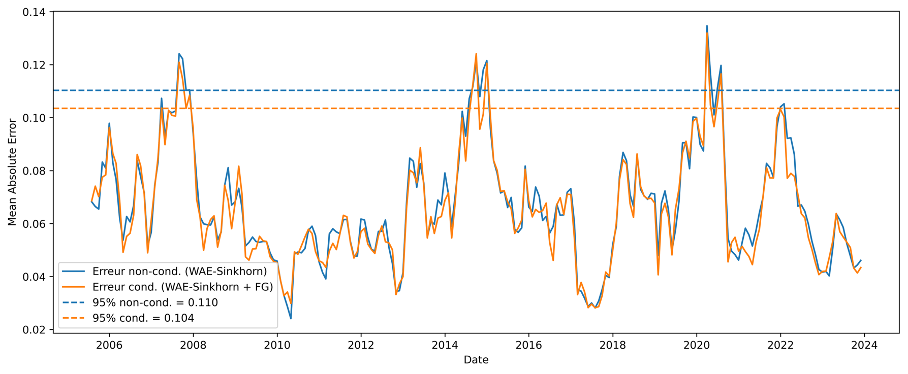
\includegraphics[width=0.9\linewidth]{images/results_ct.png}
    \caption{Erreurs de reconstruction superposées des modèles conditionnel et non conditionnel (court terme).}
    \label{fig:vae_lstm_short_term}
\end{figure}

\subsubsection{Effet de confirmation et de validation des signaux du marché}

Même si la FG n’apporte pas d’information supplémentaire significative dans la dynamique immédiate du stress systémique, elle joue un rôle important de signal de confirmation. La communication explicite de la banque centrale valide ou nuance les anticipations spontanées du marché, renforçant la crédibilité des prévisions économiques et financières.\\

Pour le régulateur, cela réduit l’incertitude liée à la prise de décision, en offrant une source d’information officielle et transparente, indispensable notamment dans des périodes de forte volatilité. Ainsi, même sans gains significatifs en termes de prédiction, la FG facilite la stabilité des anticipations, contribuant à limiter les mouvements excessifs des marchés. Ainsi, la FG peut atténuer les asymétries d’information entre les différents acteurs du marché et entre les agents économiques et le régulateur. À court terme, la disponibilité de signaux clairs issus de la politique monétaire permet une meilleure coordination des décisions, évitant que certains agents n’aient un avantage informationnel indu, facteur de volatilité et d’instabilité.\\

Cela peut avoir un impact indirect mais non négligeable sur le stress systémique, en limitant les comportements d’anticipation extrêmes ou les réactions disproportionnées à des rumeurs ou événements exogènes.

\subsubsection{Effet stabilisateur par la gestion des attentes}

La Forward Guidance contribue à orienter les anticipations des marchés financiers, même à court terme, en ancrant les attentes sur l’évolution future des conditions monétaires. Cette ancre comportementale réduit la probabilité d’ajustements brusques et inattendus, ce qui, en retour, diminue la probabilité d’une montée rapide du stress systémique. Pour le régulateur, c’est un outil précieux permettant de moduler les comportements de marché, notamment dans les phases de transition économique ou de crise naissante, en assurant une certaine fluidité dans les mécanismes de transmission de la politique monétaire.\\

Même si les marchés anticipent rapidement les chocs, la communication de la banque centrale par la FG peut influencer les conditions de liquidité à court terme, par exemple en rassurant les investisseurs sur la continuité du soutien monétaire. Cette influence indirecte sur les spreads de crédit, la volatilité ou les volumes échangés peut moduler le stress systémique, bien que cet effet ne soit pas directement observable dans la reconstruction statistique des signaux latents.

\subsubsection{Limites liées à la rapidité d’intégration des marchés}

La faible amélioration observée de la FG dans la reconstruction à court terme s’explique notamment par la sophistication et la rapidité d’adaptation des marchés financiers. Ceux-ci, en particulier les acteurs professionnels, intègrent très rapidement les informations publiques, rendant la FG redondante à ces horizons temporels.\\

Cela suggère que la valeur ajoutée de la FG réside davantage dans les horizons intermédiaires à longs termes, où la communication peut guider les anticipations et influencer durablement les comportements de marché, plutôt que dans la simple capacité à réduire les erreurs de prévision immédiates.

\subsubsection{Importance stratégique de la Forward Guidance dans la gestion des crises}

Enfin, même à court terme, la FG peut jouer un rôle stratégique en période de crise ou d’instabilité élevée. La communication claire et cohérente de la banque centrale peut prévenir des réactions de panique, en stabilisant les anticipations et en assurant aux marchés que des mesures de soutien sont en place ou envisagées. Cette fonction stabilisatrice, bien que difficile à quantifier dans les modèles à court terme, est essentielle pour le régulateur, qui doit non seulement comprendre le stress systémique, mais aussi agir pour le contenir.\\

À court terme, bien que la Forward Guidance ne semble pas améliorer significativement la capacité de reconstruction ou d’anticipation du stress systémique par rapport aux dynamiques endogènes du marché, ses effets pour le régulateur ne se limitent pas à la seule prédiction. Elle joue un rôle clé dans la réduction des incertitudes, la stabilisation des anticipations, la réduction des asymétries d’information, et la gestion des comportements de marché, particulièrement dans les phases critiques. Ces fonctions sont cruciales pour assurer la résilience du système financier, et justifient pleinement le recours à la Forward Guidance comme un outil complémentaire de la politique monétaire, même à court terme.\\

En définitive, si la Forward Guidance n’améliore que marginalement la qualité statistique des reconstructions du stress systémique à très court terme, elle joue néanmoins un rôle non négligeable dans la régulation qualitative des comportements de marché. En renforçant la lisibilité des intentions de la banque centrale, en réduisant les asymétries d’information et en stabilisant les anticipations, elle contribue à la résilience du système financier, même lorsqu’elle ne modifie pas directement les dynamiques observables du stress. Toutefois, ces effets demeurent limités par la rapidité d’intégration des marchés, ce qui tend à atténuer la portée immédiate des signaux de Forward Guidance. Il convient désormais de s’interroger sur l’effet différé de cette communication stratégique, en élargissant l’horizon temporel d’analyse. L’objectif est de déterminer si, au-delà de la réaction instantanée des marchés, la Forward Guidance parvient à façonner plus durablement les anticipations et à influencer la trajectoire latente du stress systémique. C’est ce qui est exploré dans la section suivante, consacrée à l’impact à moyen terme.

\subsection{Impact à moyen terme}

À l’horizon de 30 jours (considéré comme moyen terme), les effets différés de la communication de la BCE commencent à se manifester comme le montre la \autoref{fig:vae_lstm_mid_term}. Contrairement au court terme, où les modèles conditionnel et non conditionnel présentent des erreurs de reconstruction presque superposées, on observe ici une divergence plus marquée entre les deux dynamiques. En particulier, le modèle conditionnel  affiche une plus grande variabilité, avec des épisodes d’augmentation localisée de l’erreur — notamment durant les périodes de crise intense, comme la crise des dettes souveraines (2009–2015) et les turbulences associées à la pandémie de COVID-19 (2020–2021).

\begin{figure}[H]
    \centering
    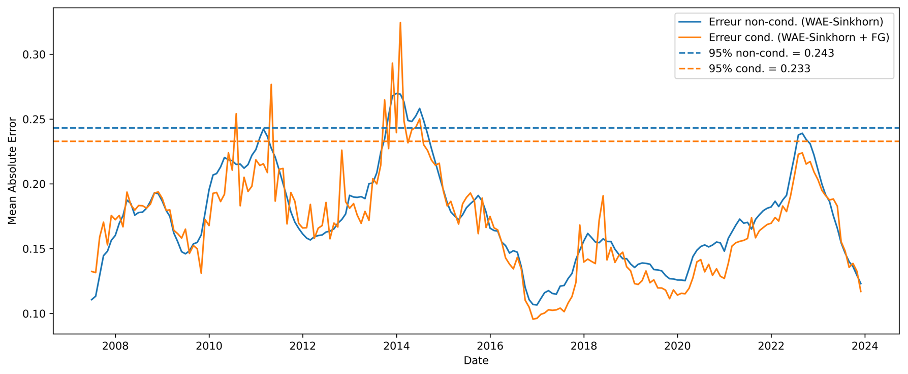
\includegraphics[width=0.9\linewidth]{images/results_mt.png}
    \caption{Erreurs de reconstruction superposées des modèles conditionnel et non conditionnel (moyen terme).}
    \label{fig:vae_lstm_mid_term}
\end{figure}

Bien que la moyenne des erreurs conditionnelles (MAE à 95\%) soit légèrement inférieure à celle du modèle non conditionné (0.233 vs 0.243), cette amélioration globale cache une instabilité structurelle : la courbe orange présente de fortes oscillations, surtout en contexte de stress économique, ce qui laisse entrevoir une difficulté du modèle à tirer parti de la FG lorsque le régime informationnel devient incertain.

\subsubsection{Un signal informatif, mais instable dans les phases de crise}

Ce comportement erratique du modèle conditionnel s’explique par plusieurs facteurs, d'une part, la variabilité accrue du discours en période de crise, durant les épisodes de forte incertitude macroéconomique, la FG devient souvent plus fréquente, plus nuancée et potentiellement plus ambiguë. D'autre part, la BCE ajuste son ton, introduit des précautions oratoires ou des formulations conditionnelles (« data-dependent », « à un rythme approprié », etc.), ce qui complique l’encodage sémantique fiable de la tonalité du discours. Le message devient moins clair et donc plus difficile à traduire dans l’espace latent vectoriel utilisé par les modèles conditionnels.\\

Ensuite, le décalage entre discours et action en situation de stress, la communication peut prendre une valeur stratégique pour temporiser les attentes, rassurer les marchés, gagner du temps. Cela peut produire une dissociation entre les intentions exprimées et les politiques effectivement mises en œuvre, créant un bruit informationnel qui altère la cohérence des projections basées sur la FG.\\

Cela est aussi dû à la réception biaisée ou instable des marchés. L’efficacité de la Forward Guidance repose sur sa crédibilité et sur la capacité des agents économiques à l’intégrer rationnellement dans leurs anticipations. Or, en période de crise, les comportements deviennent plus erratiques (effets de panique, mimétisme, changement de régime d’anticipation), réduisant la capacité de la FG à ancrer efficacement les attentes. Les marchés peuvent mal interpréter les signaux ou accorder davantage de poids aux indicateurs conjoncturels qu’aux intentions déclarées.\\

Enfn, la fragmentation sémantique dans les discours en période de crise est présente. Le discours de la BCE devient souvent moins unifié, avec une diversité de porte-parole (membres du Directoire, présidente, gouverneurs nationaux), chacun tenant un discours parfois légèrement divergent. Cette hétérogénéité de tonalité rend le signal agrégé plus difficile à interpréter pour les modèles d’apprentissage automatique.

\subsubsection{Un signal potentiellement contre-productif à moyen terme}

Dans ces conditions, la Forward Guidance peut devenir moins informative, voire contre-productive, à l’horizon de 30 jours. Les erreurs de reconstruction plus élevées dans certaines phases reflètent une situation paradoxale où l’ajout d’information exogène (ici la FG) ne réduit pas l’incertitude, mais au contraire accroît l’instabilité des prédictions du modèle.\\

Cela peut être interprété comme le retour d’un bruit communicationnel, où la complexité sémantique dépasse la capacité des encodeurs à extraire un signal directionnel robuste. Autrement dit, le modèle apprend une représentation « instable » du stress latent, trop influencée par des signaux discursifs ambigus ou contradictoires.

\subsubsection{Implications stratégiques pour les régulateurs}

Pour la BCE et les autres autorités monétaires, ces résultats soulèvent plusieurs enjeux stratégiques. Il ya clairement une nécessité de clarté accrue en période de crise : les régulateurs doivent veiller à délivrer une communication plus homogène, cohérente et lisible. Cela suppose de limiter les signaux contradictoires, d’harmoniser les discours entre les membres de l’institution, et d’éviter l’usage excessif de formulations conditionnelles qui ajoutent de la complexité sémantique.\\

En ce qui concerne l'encadrement du rôle de la FG dans les outils de gestion de crise, il ne faut pas surévaluer la capacité de la FG à stabiliser les anticipations à moyen terme durant une crise. Son efficacité diminue lorsque le bruit informationnel augmente. En ce sens, la FG doit être complémentaire à des actions crédibles, mesurables et rapides, et non un substitut à l’action monétaire.\\

Il est également possible de voir que la Forward Guidance n’est efficace que si elle s’inscrit dans une trajectoire crédible, soutenue par des décisions concrètes. Les écarts entre paroles et actes dégradent rapidement l’impact du discours, comme le montre l’augmentation de l’erreur conditionnelle dans les périodes où la politique monétaire est perçue comme hésitante ou tardive.\\

L'importance du contexte de réception pour la FG n’est pas perçue de manière uniforme dans tous les régimes économiques. Les régulateurs doivent intégrer cette réalité dans leur stratégie de communication : un même message peut être stabilisateur en période calme, mais source de confusion en période de stress. La Forward Guidance commence à produire un effet différé sur les dynamiques latentes du stress, mais cet effet est fortement dépendant du régime économique. En période de stabilité, la FG peut enrichir utilement l’information intégrée dans les modèles. En revanche, lors des crises, elle peut devenir difficile à encoder, instable, voire contre-productive. Cela plaide pour une utilisation contextualisée, prudente et stratégiquement coordonnée de cet instrument de communication, et pour un arbitrage intelligent entre clarté, cohérence et crédibilité.\\

Ces résultats à moyen terme révèlent une dynamique plus ambivalente de la Forward Guidance. Bien qu’un effet différé soit perceptible sur la trajectoire du stress systémique, sa stabilité et sa lisibilité s’amenuisent dès lors que le contexte devient incertain ou marqué par des tensions économiques aiguës. L’introduction du signal exogène issu des discours de la BCE, loin de toujours clarifier la trajectoire anticipée, peut en certaines circonstances introduire une volatilité supplémentaire dans la modélisation du stress. Cela souligne les limites de la Forward Guidance lorsqu’elle n’est pas adossée à une stratégie de communication cohérente et à une action monétaire perçue comme crédible. Dès lors, son efficacité ne dépend pas uniquement de sa fréquence ou de sa tonalité, mais surtout de la manière dont elle est perçue et interprétée par les marchés dans un environnement donné. Il reste à déterminer si, sur des horizons plus longs, la Forward Guidance parvient à dépasser ces limitations conjoncturelles. En d'autres termes, son impact s’inscrit-il dans une logique d’ancrage progressif des anticipations ou s’efface-t-il au fil du temps sous l’effet des chocs exogènes ? Il est dorénavant proposé d’examiner cette question en analysant les dynamiques observées à long terme.

\newpage

\subsection{Impact à long terme}

Les résultats empiriques obtenus à l’horizon de six mois dans la \autoref{fig:vae_lstm_long_term} mettent clairement en évidence la supériorité explicative du modèle conditionnel, c’est-à-dire celui intégrant l’indice directionnel de FG. L’écart entre les erreurs absolues moyennes (MAE à 95\%) est significatif : 0.166 pour le modèle conditionnel contre 0.213 pour le modèle non conditionné. Ce gain de performance reflète une capacité accrue à anticiper les évolutions latentes du stress systémique lorsque le modèle est informé par la tonalité des discours de la BCE.

\begin{figure}[H]
    \centering
    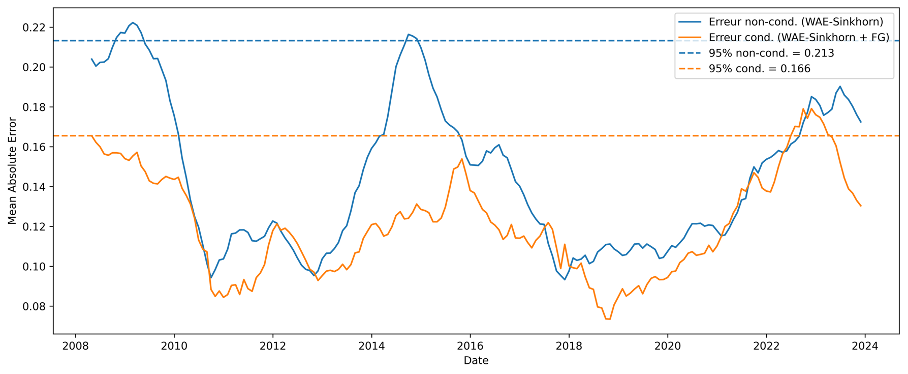
\includegraphics[width=0.9\linewidth]{images/results_lt.png}
    \caption{Erreurs de reconstruction superposées des modèles conditionnel et non conditionnel (long terme).}
    \label{fig:vae_lstm_long_term}
\end{figure}

Plus encore, l’analyse visuelle des trajectoires révèle des décalages temporels marqués entre les deux modèles, en particulier sur certaines périodes structurellement instables ou marquées par des transitions de régime monétaire — notamment entre 2011 et 2016 (phase post-crise souveraine en zone euro) et 2021 à 2023 (retour de l’inflation et réorientation vers une politique monétaire plus restrictive). Dans ces moments charnières, le modèle conditionnel parvient non seulement à anticiper l’intensification du stress, mais aussi à capter ses fluctuations différées, en lien avec les ajustements graduels des anticipations de marché.

\subsubsection{Un signal sémantique à effet différé : transmission longue de la FG}

L’analyse de ces résultats suggère une propriété centrale de la Forward Guidance : son impact sur le stress systémique est temporellement différé. Contrairement aux interventions monétaires directes (taux, opérations de refinancement, achats d’actifs), qui peuvent produire des effets immédiats sur la liquidité ou les prix d’actifs, la FG opère principalement via les anticipations. Les canaux par lesquels la FG influence le stress latent sont fondamentalement intertemporels.\\

D'abord, le canal des anticipations de taux futurs avec les déclarations orientent les croyances des agents économiques sur la trajectoire future des taux directeurs. Ces ajustements progressifs des anticipations affectent les décisions d’investissement, de crédit et de couverture avec un temps de latence significatif. Ensuite, le canal de crédibilité institutionnelle : une communication cohérente et récurrente renforce la confiance des marchés dans la capacité de la BCE à agir en cohérence avec ses annonces. Cette confiance ne se construit pas instantanément, mais s’accumule sur plusieurs mois, expliquant pourquoi l’indicateur directionnel devient plus prédictif à long terme. Enfin, le canal d’ancrage des anticipations d’inflation et de risque systémique où la FG contribue à stabiliser les anticipations macroéconomiques de long terme (inflation, croissance, volatilité financière), ce qui modère ex post la survenance de chocs de stress à horizon éloigné.\\

Ainsi, la baisse marquée de l’erreur du modèle conditionnel à 6 mois s’explique par le fait que la FG agit comme un indicateur avancé des futurs déséquilibres systémiques, mais que son impact ne se matérialise que dans un second temps — après diffusion dans les comportements d’allocation de portefeuille, les ajustements de bilans bancaires ou encore la reconfiguration des régimes de risque.

\subsubsection{Rôle différencié de la FG selon le régime macro-financier}

Les résultats montrent également que la valeur informative de la FG varie selon le contexte et le régime. En période de stabilité (par exemple 2013–2016), la FG joue un rôle de signal anticipatif puissant, guidant les marchés de manière douce et prévisible. Les discours de la BCE ont alors un effet de stabilisation stratégique, permettant aux acteurs de se repositionner graduellement, ce qui se traduit par une réduction effective du stress latent.\\

En période de transition ou de tension sous-jacente (par exemple 2021–2023), la FG agit comme un révélateur de rupture. La sémantique change, les mots employés deviennent plus restrictifs, ce qui précède — parfois de plusieurs mois — les inflexions effectives de la politique monétaire. Ces inflexions sont captées par les marchés dans un second temps, ce qui explique pourquoi le modèle conditionnel permet de détecter des ruptures anticipées dans les dynamiques du stress.\\

En période de crise ouverte, la FG ne semble pas être la source principale de variation du stress comme montré précédemment à moyen terme. Toutefois, à long terme, une communication résolument accommodante ou un changement de cap affirmé peut finir par rassurer les marchés, induisant une décrue progressive du stress systémique (exemple : les annonces de Draghi en 2012 « whatever it takes »).

\subsubsection{Implications de politique économique}

Ces résultats ont plusieurs implications fondamentales pour les régulateurs, en particulier les banques centrales et les autorités macroprudentielles. La Forward Guidance est un instrument stratégique de moyen-long terme : elle ne doit pas être évaluée uniquement à l’aune de ses effets instantanés. Son efficacité se manifeste dans sa capacité à préparer les ajustements structurels, à façonner les anticipations, et à ancrer la trajectoire future des politiques économiques.\\

La stabilité, la clarté et la cohérence de la communication sont cruciales, plus la communication est lisible, plus l’effet différé est net. Cela appelle une gestion rigoureuse de la séquence des discours, un encadrement strict des divergences narratives internes à l’institution, et un suivi continu des effets sémantiques.\\

La FG peut être utilisée comme indicateur avancé de stress latent dans une logique de prévention : au-delà de sa fonction de transmission, la tonalité agrégée des discours constitue un signal exploitable pour calibrer les politiques macroprudentielles, anticiper les points de rupture potentiels ou déclencher des mesures de soutien préventives. Aussi, l’efficacité différée de la FG invite à combiner les horizons de pilotage : une politique monétaire efficace doit s’articuler sur plusieurs niveaux temporels : instruments à effet immédiat (taux, opérations de marché), mécanismes de stabilisation de moyen terme (filet de sécurité bancaire, interventions ciblées), et communication de long terme visant les anticipations.\\

L’analyse empirique montre que, parmi les différents horizons temporels étudiés, c’est à long terme que la Forward Guidance révèle toute sa puissance explicative. Sa nature discursivement anticipative, son ancrage institutionnel et sa capacité à structurer les anticipations macro-financières en font un instrument d’orientation des comportements économiques plus qu’un outil de réaction immédiate. Les performances du modèle conditionnel indiquent que la tonalité des discours de la BCE est fortement corrélée, avec un décalage temporel, aux évolutions latentes du stress systémique. Cela confirme empiriquement la dimension stratégique de la communication monétaire, non seulement comme outil d’accompagnement, mais aussi comme mécanisme d’amortissement et de pilotage à horizon long dans la gestion des risques systémiques.\\

Ainsi, l’analyse à long terme met clairement en lumière la dimension stratégique de la Forward Guidance dans le pilotage du stress systémique. Contrairement aux horizons plus courts, où ses effets peuvent être atténués par la rapidité d’ajustement des marchés, son rôle se révèle pleinement lorsqu’on observe les dynamiques financières sur des périodes étendues. La communication monétaire, lorsqu’elle est cohérente, lisible et inscrite dans un cadre institutionnel stable, constitue un levier puissant pour orienter les anticipations collectives, amortir les transitions de régime et stabiliser progressivement les équilibres systémiques. Le caractère différé de son efficacité impose toutefois une vigilance accrue quant à la qualité du signal émis, à la clarté du message délivré et à la synchronisation entre les intentions exprimées et les instruments mobilisés. L’analyse appelle désormais une réflexion plus normative : comment les régulateurs, et en particulier la Banque centrale européenne, peuvent-ils optimiser l’usage de la Forward Guidance dans leur arsenal d’intervention ? Quelles recommandations concrètes peut-on formuler en matière de communication, de coordination inter-institutionnelle ou de conception des outils macroprudentiels ? La section suivante propose de répondre à ces interrogations en formulant un ensemble de recommandations opérationnelles à destination des autorités monétaires et de supervision.

\subsection{Recommandations opérationnelles pour la BCE et les autorités macroprudentielles}

Les résultats empiriques présentés dans ce chapitre ont mis en évidence le rôle différencié de la Forward Guidance (FG) selon les horizons temporels et les régimes macro-financiers. Si son effet est limité à court terme, la FG se révèle particulièrement efficace à moyen et long termes, notamment en tant qu’ancre anticipative des comportements de marché. Afin de renforcer cette efficacité, plusieurs recommandations opérationnelles peuvent être formulées à destination de la Banque Centrale Européenne (BCE) et, plus largement, des autorités chargées de la stabilité financière. Ces recommandations visent à améliorer la clarté, la crédibilité et la cohérence de la communication monétaire, en articulant plus étroitement les messages sémantiques et les instruments de politique économique.

\subsubsection{Renforcer la cohérence et la traçabilité de la communication monétaire}

Il a été observé que la fragmentation de la communication institutionnelle, notamment dans les phases de crise, tend à générer du bruit sémantique, compromettant la lisibilité des signaux monétaires. Cette hétérogénéité, souvent causée par la multiplicité des porte-parole ou par des divergences narratives entre les membres du Conseil des gouverneurs, se traduit par une volatilité accrue du stress latent. Afin de limiter ce phénomène, une harmonisation de la voix institutionnelle doit être systématiquement recherchée. Cela peut passer par l’instauration d’un calendrier officiel structurant les prises de parole prioritaires (notamment celles de la présidence ou du chef économiste) et par la définition ex ante de lignes directrices sémantiques à respecter dans les communications publiques.

Par ailleurs, la crédibilité de la FG pourrait être consolidée en l’adossant à des jalons d’action observables. Il serait opportun que les annonces de politique monétaire fassent explicitement référence à des seuils ou des indicateurs vérifiables, tels que le taux d’inflation sous-jacent, la dispersion des primes de risque souverain ou le niveau d’output gap. L’adoption d’une matrice condition–action, même simplifiée, renforcerait la transparence du processus de décision, tout en préservant une marge d’ajustement. Une communication exprimée sous forme de plages cibles, plutôt que de points fixes, permettrait d’éviter toute rigidité excessive, tout en maintenant une orientation stratégique.

\subsubsection{Mettre en place un système de suivi sémantique intégré et réactif}

L’efficacité de la communication de politique monétaire repose en grande partie sur la clarté, la cohérence et la stabilité des signaux transmis. Dans cette perspective, il apparaît essentiel de doter l’autorité monétaire d’un système de suivi sémantique capable de capter en temps réel les inflexions discursives et d’en mesurer l’impact potentiel sur les anticipations de marché. Une telle infrastructure permettrait d’objectiver le contenu sémantique des discours, d’assurer leur alignement avec les objectifs stratégiques de la politique monétaire, et de prévenir les dissonances narratives susceptibles d’accroître l’incertitude ou de générer un stress financier inutile.\\

À cet effet, il est proposé la mise en place d’un tableau de bord dédié à l’analyse de la Forward Guidance, dont la conception pourrait s’inspirer des méthodes développées dans la présente étude. Ce tableau de bord intégrerait plusieurs indicateurs complémentaires, actualisés à chaque nouvelle publication institutionnelle. Tout d’abord, une mesure directionnelle, analogue à l’indice $z_t$, permettrait de quantifier la tonalité sémantique de chaque discours selon un axe latent allant de l’accommodant au restrictif. Cette mesure serait calculée sur la base d’un encodage sémantique automatisé, projeté sur une direction vectorielle construite à partir de phrases d’ancrage générées et validées selon une procédure standardisée. En complément, un indicateur de dispersion inter-locuteur pourrait être introduit afin de mesurer l’hétérogénéité des positions discursives entre les différents membres du Conseil des gouverneurs. Ce coefficient de dispersion, calculé par exemple comme l’écart-type des scores $z_t$ sur une période donnée, permettrait d’identifier les périodes où les signaux envoyés aux marchés apparaissent ambigus ou contradictoires. Une telle situation est généralement corrélée à une perte de lisibilité de la stratégie monétaire, et peut induire une volatilité excessive, comme le suggèrent les résultats empiriques observés à moyen terme dans les phases de crise.\\

Par ailleurs, une métrique de stabilité temporelle devrait être ajoutée, par exemple sous la forme d’une variance mobile des scores sémantiques sur un horizon glissant de plusieurs semaines ou mois. Cette mesure permettrait de suivre la cohérence inter-temporelle de la communication, et de détecter d’éventuels glissements discursifs non intentionnels. Une montée soudaine de la variance sémantique constituerait ainsi un signal d’alerte, susceptible de déclencher une intervention corrective.\\

Afin de donner une portée opérationnelle à ce tableau de bord, il conviendrait d’y associer un mécanisme de gouvernance. Il est proposé que des seuils d’alerte soient fixés pour chacun des indicateurs, de manière à identifier les situations nécessitant une réponse institutionnelle. En cas de dépassement de ces seuils, un comité éditorial interne pourrait être mobilisé. Sa mission consisterait à analyser les causes de la divergence sémantique, à recommander des ajustements de formulation, voire à coordonner les prochaines prises de parole afin de rétablir l’unité narrative. Ce comité, composé de représentants de la direction de la communication, du département de politique monétaire et du secrétariat général, jouerait un rôle central dans la régulation qualitative de la FG.\\

Parallèlement, il apparaît souhaitable d’exploiter les avancées récentes en NLP pour automatiser une partie de ce suivi. L’usage de modèles de type transformeurs, notamment BERT, Mamba ou Llamba, permettrait de mettre en œuvre des outils de surveillance sémantique en temps réel. Grâce à des techniques d’attention contextuelle et de classification latente, il deviendrait possible de détecter automatiquement les glissements de tonalité, les ruptures stylistiques, ou encore les contradictions implicites entre différents segments de discours. Cette surveillance algorithmique, couplée à une interface visuelle interactive, constituerait un appui précieux pour les responsables de la communication stratégique. Toutefois, le pilotage qualitatif de la FG ne saurait se limiter à un contrôle ex ante. Une démarche d’évaluation ex post s’impose, à l’image de ce qui est pratiqué pour les outils non conventionnels tels que les programmes d’achats d’actifs. Il serait donc recommandé de publier, à intervalles réguliers (par exemple semestriellement), un rapport d’évaluation de la communication monétaire. Ce rapport relierait, à l’aide de méthodes économétriques rigoureuses, les caractéristiques sémantiques des discours publiés à l’évolution des indicateurs de stress systémique, des spreads de taux d’intérêt, ou encore de la volatilité implicite sur les marchés financiers.\\

En cas d’écart significatif entre les effets attendus de la FG et les dynamiques observées sur les marchés, une révision des stratégies discursives pourrait être envisagée. Cette révision porterait soit sur le contenu (simplification du message, clarification des intentions), soit sur la forme (choix du canal de communication, fréquence des publications, identité du parleur). Ainsi, le lien entre analyse sémantique et pilotage stratégique serait pleinement institutionnalisé.

\subsubsection{Intégrer la Forward Guidance dans une architecture de réponse coordonnée aux chocs}

Les résultats empiriques ont révélé que, durant les périodes de forte instabilité, la FG ne produit ses effets que lorsqu’elle est accompagnée de mesures tangibles. La communication verbale, lorsqu’elle est isolée, tend à perdre de sa capacité d’ancrage. Dès lors, une coordination renforcée entre FG et instruments de liquidité s’impose. Les annonces de FG gagneraient à être systématiquement couplées à la publication de calendriers d’intervention, à l’annonce des montants prévus ou à la réactivation de dispositifs ciblés tels que les T-LTRO, PELTRO ou lignes de swap. Cette approche conjointe permettrait d’amplifier l’effet de signal et de renforcer la crédibilité de la trajectoire annoncée. Par ailleurs, la FG devrait être articulée de manière plus explicite avec la politique macroprudentielle. Les outils tels que le coussin contracyclique, les réserves obligatoires différenciées ou les orientations sectorielles devraient être calibrés en cohérence avec les signaux sémantiques envoyés par la BCE. Une telle coordination réduirait le risque de messages contradictoires et renforcerait l’efficacité globale du cadre de stabilisation financière. Enfin, les résultats suggèrent qu’une adaptation de la granularité temporelle de la FG est nécessaire. Étant donné l’efficacité différée de la communication observée à l’horizon de six mois, il conviendrait de privilégier une guidance explicite pour les thématiques de moyen et long termes (politique de bilan, trajectoire des taux d’intérêt nominaux), tout en maintenant une guidance plus qualitative ou contingente à court terme. Cette flexibilité temporelle permettrait d’éviter les effets de sur-interprétation immédiate, tout en assurant un encadrement stratégique durable des anticipations. L’ensemble de ces recommandations vise à faire de la Forward Guidance non plus seulement un vecteur d’intentions, mais un instrument intégré à l’architecture de stabilisation macro-financière. Lorsqu’elle est bien faite, la communication de la BCE peut devenir un puissant levier de réduction du stress systémique, en particulier sur les horizons temporels où les canaux de transmission sont les plus actifs.

\newpage

Ce chapitre a proposé une architecture intégrée pour analyser empiriquement l’impact de la Forward Guidance sur le stress systémique, à l’aide de méthodes avancées en traitement automatique du langage naturel et en modélisation de séries temporelles. L’objectif principal était d’établir une passerelle rigoureuse entre les signaux sémantiques émis par la Banque centrale européenne et les dynamiques latentes de vulnérabilité financière, en montrant que le langage de politique monétaire, loin d’être un simple artefact rhétorique, constitue une variable économique de premier plan.\\

La première étape de cette analyse a consisté à encoder la tonalité des discours de politique monétaire. Pour cela, un indicateur directionnel de Forward Guidance a été construit en projetant chaque document textuel dans un espace sémantique latent, à l’aide de modèles de langage pré-entraînés. Des architectures distinctes, telles que ModernBERT, Mamba, Mamba-2 et Llamba, ont été mobilisées pour produire des représentations vectorielles de haute dimension, à partir desquelles des scores directionnels ont été extraits par projection dans un axe discursif structuré allant du registre restrictif vers l’orientation expansionniste. L’évaluation comparative de ces représentations, via des régressions Ridge appliquées à un indicateur de stress financier comme le CISS, a permis de sélectionner les encodeurs offrant la meilleure capacité explicative du stress systémique pour Mamba. Sur cette base, un modèle d’autoencodeur Wasserstein-LSTM conditionnel a été développé afin de capturer les dynamiques structurelles du stress latent. Ce modèle s’appuie sur la régularisation de l’espace latent via une contrainte de transport optimal, assurant une géométrie probabiliste cohérente, tout en permettant d’intégrer de manière conditionnelle les signaux exogènes issus de la Forward Guidance. Cette architecture a été appliquée aux séries temporelles financières découpées en fenêtres glissantes, afin d’en reconstruire l’évolution à différents horizons temporels, en comparant les erreurs issues d’un modèle conditionné par la FG à celles d’un modèle non informé.\\

Les résultats empiriques ont révélé une hétérogénéité significative des effets de la Forward Guidance selon l’horizon temporel. À très court terme, la valeur ajoutée de la communication apparaît limitée : les marchés financiers, par leur nature hautement réactive, semblent intégrer rapidement les signaux disponibles, rendant la FG redondante d’un point de vue prédictif. Toutefois, cette observation ne doit pas masquer le rôle stratégique que joue la FG dans la réduction des incertitudes, la stabilisation des anticipations, et la prévention des asymétries informationnelles. La FG agit comme une boussole narrative, utile pour encadrer les interprétations de marché même lorsqu’elle ne modifie pas substantiellement les trajectoires. À moyen terme, les effets deviennent ambigus. En période de stabilité relative, la FG peut continuer à guider les anticipations de manière efficace. En revanche, en période de crise ou d’incertitude accrue, la complexité sémantique des discours, (due à l’usage accru de formulations conditionnelles, à la multiplicité des porte-parole, ou à des ajustements tactiques dans la communication) peut altérer la lisibilité du signal. Cette dégradation du contenu informationnel se traduit, dans les modèles conditionnels, par une instabilité accrue des reconstructions, voire par une perte de performance prédictive. Ce paradoxe – où un excès de communication nuit à la capacité d’anticipation souligne les limites opérationnelles de la Forward Guidance en contexte de stress aigu. C’est à long terme que la puissance explicative de la Forward Guidance s’affirme avec le plus de netteté. Les modèles conditionnels surpassent de manière robuste les versions non conditionnelles, tant en termes d’erreur moyenne que de capacité à détecter les transitions de régime. Cette supériorité s’interprète comme la manifestation différée d’un canal d’anticipation structurel : en orientant les croyances sur les trajectoires futures de la politique monétaire, la FG influence les décisions d’investissement, la gestion des risques, et les arbitrages de portefeuille, avec un effet amorti mais cumulatif. L’ancrage des anticipations opère donc dans un espace-temps élargi, compatible avec la temporalité des ajustements macro-financiers.\\

L’utilisation d’architectures issues du deep learning se justifie donc par la nature même des données mobilisées et des dynamiques recherchées. Les méthodes traditionnelles, fondées sur des hypothèses linéaires ou paramétriques fortes, se heurtent à la complexité structurelle des séries financières et à la richesse sémantique des discours de politique monétaire. En effet, le langage de la Forward Guidance ne suit pas une syntaxe standardisable ni des relations fixes entre variables, mais mobilise des tournures implicites, conditionnelles ou stratégiques, difficilement capturables par des modèles linéaires classiques. De même, les trajectoires du stress systémique obéissent à des régimes multiples, parfois latents, dont les transitions ne peuvent être appréhendées de manière satisfaisante par des approches stationnaires. En combinant des modèles de langage non supervisés, capables de structurer l’information textuelle dans des espaces latents complexes, avec des autoencodeurs dynamiques régularisés par le transport optimal, le deep learning offre une capacité unique à extraire, intégrer et projeter des signaux discontinus et multidimensionnels. Ce paradigme permet non seulement une meilleure reconstruction des dynamiques observées, mais aussi une modélisation plus réaliste des mécanismes d’anticipation et de propagation du stress. Il ne s’agit donc pas d’un simple choix technique, mais d’un cadre méthodologique cohérent avec l’hypothèse d’une économie informationnellement dense, où la communication devient une variable structurelle à part entière.\\

Ces résultats soulignent le caractère intertemporel de la FG, qui se distingue fondamentalement des instruments traditionnels de politique monétaire. Là où les taux d’intérêt ou les programmes d’achat produisent des effets immédiats, la FG agit par diffusion lente à travers les canaux de communication, de crédibilité et de coordination. Elle constitue un levier de stabilisation dont l’efficacité repose sur la cohérence narrative, la lisibilité des signaux, et l’alignement entre intentions déclarées et actions réelles. En définitive, ce chapitre apporte une double contribution : méthodologique, en proposant une chaîne de traitement unifiée combinant NLP avancé et modélisation du stress latent ; et empirique, en mettant en évidence la nature temporellement différée et stratégiquement conditionnée de l’impact de la Forward Guidance sur le stress systémique. Il en résulte une perspective renouvelée sur le rôle de la communication monétaire, non pas comme simple accompagnement rhétorique des décisions, mais comme instrument actif de gestion des risques financiers. Cette perspective invite à repenser la place de la FG dans les outils de régulation contemporains, et appelle à une réflexion approfondie sur les conditions de son efficacité. C’est à cette réflexion opérationnelle que s'est consacré cette étude.